%% see also NotesICA.tex in SS2013
%% add matrix version to PCA methods (see handwritten notes in script)?

\newpage 						% for visual reasons
\section{Projection Methods}
Projection methods provide important tools for high-dimensional datasets
\begin{figure}[h]
  \centering
  \begin{tabular}{c c}
    \raisebox{-2cm}{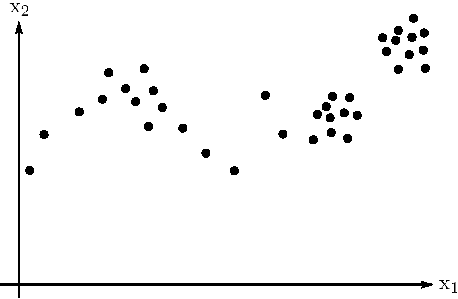
\includegraphics[width=5cm]{section2_fig1}} & 
    \parbox{5.6cm}{$p$ observations with $N$ dims.:\\ 
    $\big\{ \vec{x}^{(1)}, \; \vec{x}^{(2)}, \; \ldots, \; \vec{x}^{(p)} \in \mathbb{R}^N \big\}$}
%     $\big\{ \vec{x}^{(\alpha)} \big\}, \alpha = 1, \ldots, p; \quad \vec{x}^{(\alpha)} \in \mathbb{R}^N$}
  \end{tabular}
  \caption{Projection and clustering methods for multidimensional data}
  \label{tab:scenario-proj-meth}
\end{figure}



\subsection{Principal Component Analysis}\label{sec:PCA}
% -----------------------------------------------------------------------------

\subsubsection{The Covariance Matrix}
observations: $\big\{ \vec{x}^{(\alpha)} \big\}, \; \alpha = 1, \ldots, p; \quad \vec{x}^{(\alpha)} \in \mathbb{R}^N$
\\\\
{\bf Feature space:}
\begin{figure}[h]
  \centering
  \includegraphics[width=8cm]{section2_fig2}  
  \caption{Data, elementary and complex features}
  \label{fig:features}
\end{figure}
\begin{figure}[h]
  \centering
  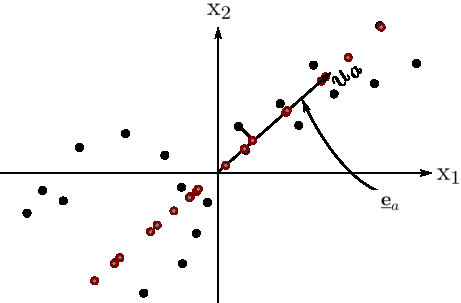
\includegraphics[width=8cm]{section2_fig2b}  
  \caption{Same data as in Fig.~\ref{fig:features}, projected onto complex feature $\vec{e}_a$ with feature values $u_a$}
  \label{fig:featuresproj}
\end{figure}
\begin{description}
\item[elementary features $\vec{e}_\mathrm{x}^{(1)}, \vec{e}_\mathrm{x}^{(2)}, \vec{e}_\mathrm{x}^{(3)}, \ldots \vec{e}_\mathrm{x}^{(N)}$:] basis vectors of unit length which correspond to the individual measurements
\item[complex feature $\vec{e}_a$:] vector of unit ($\|\vec{e}_a\|=1$) length which
  corresponds to a particular direction in feature space
\item[feature value $u_a$:] projection of observation $\vec{x}$ onto the complex feature $\vec{e}_a$
\end{description}
\begin{equation}
	\underbrace{u_a }_{ \text{{\small value}} }
	= \underbrace{ \vec{e}_a^T }_{ \text{{\small feature}} }
	\cdot \underbrace{ \vec{x} }_{ \text{{\small observation}} }
\end{equation}


\paragraph{Example -- Leptograpsus data:} Dead crabs lose their color and their sexual features -- 
Can we infer species / sex from the shells alone?
\[ \text{crabs: L. variegatis} \left\{ \begin{array}{l}
		\text{orange} \\\\
		\text{blue}
	\end{array} \right. \left\} \begin{array}{l}
		\text{two (sub-)species} \\\\
		\rightarrow \text{ male and female crabs}
	\end{array} \right.
\] \slideref{Ex: More examples on slide\\Leptograpsus data, Iris data}

\begin{itemize}
\item \emph{elementary features: }
\[ \left. \begin{array}{ll}
	\text{width of the frontal lip:} & \mathrm{x}_1 \\
	\text{width of the back:} & \mathrm{x}_2 \\
	\text{length along midline:} & \mathrm{x}_3 \\
	\text{max. width of top shell:} & \mathrm{x}_4 \\
	\text{body depth:} & \mathrm{x}_5
\end{array} \right\} \text{5-dim. feature vector} \]
\item \emph{complex features:} some direction in feature space (i.e.\ linear combination of elementary features) which is indicative of color and/or sex.
\end{itemize}

\paragraph{Moments of the set of observations:} Moments of a distribution provide important information about the location and shape of a distribution.
\\\\
First moment (sample mean/center of mass):
\begin{equation}
	\vec{m} = \frac{1}{p} \sum\limits_{\alpha = 1}^p \vec{x}^{(\alpha)}
\end{equation}
Second moments (Variances and Covariances):
\begin{equation}
	C_{ij} = \frac{1}{p} \sum\limits_{\alpha = 1}^p 
		\underbrace{ \Big( \mathrm{x}_i^{(\alpha)} - m_i \Big) }_{
			\substack{	\text{deviations from} \\
					\text{the mean}} }
		\underbrace{ \Big( \mathrm{x}_j^{(\alpha)} - m_j \Big) }_{
			\substack{	\text{component} \\
					\text{indices } i,j}}
\end{equation}
In vector notation:
\begin{equation} \tag{covariance matrix}
	\vec{C} = \frac{1}{p} \sum\limits_{\alpha=1}^p 
		  \left ( \vec{x}^{(\alpha)} - \vec{m} \right ) \left ( \vec{x}^{(\alpha)} - \vec{m} \right )^T
		% =   \big\{ C_{ij} \big\}
\end{equation}
\textbf{Note:} ''Centering'' the data\footnote{centering: subtract mean from all data points} yields
$\vec{m} = \vec{0}$ and we obtain
\begin{equation}
	C_{ij} = \frac{1}{p} \sum\limits_{\alpha = 1}^p \mathrm{x}_i^{(\alpha)}
			\mathrm{x}_j^{(\alpha)}
\end{equation}
and thus 
\begin{equation}
	\vec{C} = \frac{1}{p} \sum\limits_{\alpha=1}^p 
		   \vec{x}^{(\alpha)}\left ( \vec{x}^{(\alpha)}\right )^T
		% =   \big\{ C_{ij} \big\}
\end{equation}

\paragraph{Properties of the covariance matrix}
\[ \begin{array}{ll}
	C_{ij} = C_{ji}
	& \text{the covariance matrix is symmetric} \\\\
	i = j
	& C_{ii} = \frac{1}{p} \sum\limits_{\alpha = 1}^p \Big( 
			\mathrm{x}_i^{(\alpha)} - m_i \Big)^2 \\ 
	& \leadsto \text{ variance of the data along the elementary features }
        \vec{e}_\mathrm{x}^{(i)} \text{(variance of variable } \mathrm{x}_i
		\text{)} \\\\
	i \neq j 
	& C_{ij}: \text{ covariances} \\
	& \leadsto \text{ measure of correlations between variables} \\
	& \leadsto C_{ij} = 0 \rightarrow \text{ variables are uncorrelated} 
\end{array} \]
\begin{figure}[h]
  \centering
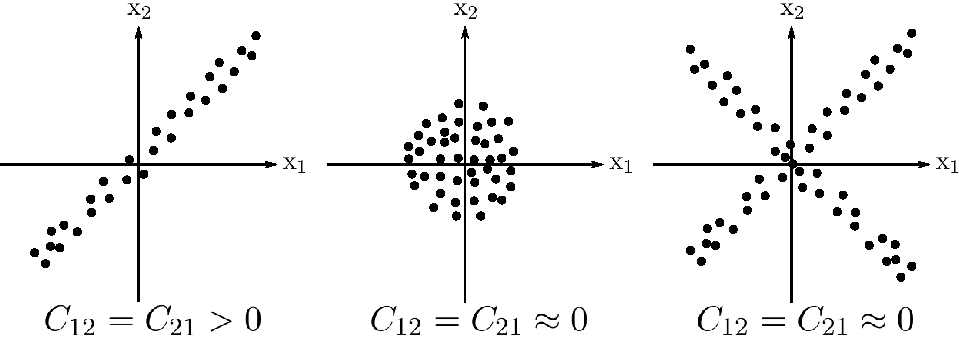
\includegraphics[width=12cm]{section2_fig3}  
\caption{Illustration of data patterns: Note that $C_{ij} = 0$ does
  \underline{not} imply that there are no dependencies between the
  variables. Clearly, $p(\mathrm{x}_1,\mathrm{x}_2) \neq
  p(\mathrm{x}_1)p(\mathrm{x}_2)$ in the third example.}
  \label{fig:correlations}
\end{figure}
\\
First moment of the data projected onto an arbitrary complex feature $\vec{e}_a$:
\begin{equation} \tag{mean}
	\begin{array}{ll}
		m_a 
		& = \frac{1}{p} \sum\limits_{\alpha = 1}^p u_a^{(\alpha)} \\\\
		& = \frac{1}{p} \sum\limits_{\alpha = 1}^p \vec{e}_a^T \cdot
			\vec{x}^{(\alpha)} \\\\
		& = \vec{e}_a^T \cdot \vec{m}
	\end{array}	
\end{equation}
Second moment along this direction:
\begin{equation} \tag{variance}
	\begin{array}{ll}
	\sigma_a^2 
	& = \frac{1}{p} \sum\limits_{\alpha = 1}^p \Big( u_a^{(\alpha)} - m_a
		\Big)^2 \\\\
	& = \frac{1}{p} \sum\limits_{\alpha = 1}^p \Big( \vec{e}_a^T
		\vec{x}^{(\alpha)} - \vec{e}_a^T \vec{m} \Big)^2 \\\\
	& = \frac{1}{p} \sum\limits_{\alpha = 1}^p \bigg\{
		\Big( \vec{e}_a^T \vec{x}^{(\alpha)} \Big)^2
		- 2 \Big( \vec{e}_a^T \vec{x}^{(\alpha)} \Big) \vec{e}_a^T
		\vec{m} + \Big( \vec{e}_a^T \vec{m} \Big)^2
		\bigg\} \\\\
	& \text{with } \vec{e}_a^T \vec{x}^{(\alpha)} = \sum\limits_{i = 1}^N
		\big( \vec{e}_a \big)_i \vec{x}_i^{(\alpha)} \text{ we obtain}
		\\\\
	& = \sum\limits_{i,j = 1}^N \big( \vec{e}_a \big)_i \frac{1}{p}
		\sum\limits_{\alpha = 1}^p \bigg\{ \mathrm{x}_i^{(\alpha)}
			\mathrm{x}_j^{(\alpha)} - \mathrm{x}_i^{(\alpha)}
			m_j - \underbrace{ \mathrm{x}_i^{(\alpha)} m_j }_{
				\substack{ = m_i x_j^{(\alpha)} \\
					\text{change of} \\
					\text{indices}} }
			+ m_i m_j \bigg\} \big( \vec{e}_a \big)_j \\\\
	& = \sum\limits_{i,j = 1}^N \big( \vec{e}_a \big)_i \bigg\{
		\underbrace{ \frac{1}{p} \sum\limits_{\alpha = 1}^p
		\Big( \mathrm{x}_i^{(\alpha)} - m_i \Big) \Big(
		\mathrm{x}_j^{(\alpha)} - m_j \Big) }_{
			= C_{ij} } \bigg\} \big( \vec{e}_a \big)_j
	\end{array}
\end{equation}
\begin{equation}
	\fbox{$ \sigma_a^2 = \vec{e}_a^T \vec{C} \vec{e}_a
	$}
\end{equation}
\textbf{Observation:} The covariance matrix determines the variance of
the data along every possible direction.

% -----------------------------------------------------------------------------

\subsubsection{The Principle of Maximal Variance}
''interesting'' complex features:
\begin{itemize}
	\itR properties of the data which vary most strongly across the data set and might therefore allow to characterize different data points
	\itR direction in feature space along which variance is maximal
		\[ \left. \begin{array}{ll}
			\fbox{$ \sigma_a^2 = \max \big( \vec{e}_a \big) $} \\\\
			\fbox{$ \vec{e}_a^2 = 1 $}
		\end{array} \right. 
		\substack{ 	\text{optimisation} \\
				\text{under constraints} } \]
\end{itemize}
Solution is found using the method of Lagrange multipliers:
\begin{equation}
	\underbrace{ \vec{e}_a^T \vec{C} \vec{e}_a }_{
		\text{objective} }
	- \underbrace{ \lambda }_{ \substack{ 	\text{Lagrange} \\
						\text{multiplier}} }
		\underbrace{ \big( \vec{e}_a^2 - 1 \big) }_{
			\text{constraints} }
	\eqexcl \max
\end{equation}
\begin{itemize}
	\itl family of solutions parametrized by $\lambda$
	\itl $\lambda$ must be chosen such that constraints are fulfilled
\end{itemize}
\begin{equation}
	f(\vec{e}_a) := \sum\limits_{i,j = 1}^N \big( \vec{e}_a \big)_i C_{ij} \big( \vec{e}_a
		\big)_j - \lambda \Bigg\{ \sum\limits_{i = 1}^N \big(
		\vec{e}_a \big)_i^2 - 1 \Bigg\} \eqexcl \max
\end{equation}
\begin{equation}
	\frac{\partial f}{\partial \big( \vec{e}_a \big)_k} \eqexcl 0
	\text{ for all components }k
\end{equation}
\begin{equation}
	\sum\limits_{j = 1}^N C_{kj} \big( \vec{e}_a \big)_j 
		+ \sum\limits_{i = 1}^N \big( \vec{e}_a \big)_i C_{ik}
		- 2 \lambda \big( \vec{e}_a \big)_k \eqexcl 0
\end{equation}
\begin{equation}
	2 \sum\limits_{j = 1}^N C_{kj} \big( \vec{e}_a \big)_j - 2 \lambda
		\big( \vec{e}_a \big)_k \eqexcl 0
		\text{ because } \vec{C} \text{ is symmetric}
\end{equation}
\begin{equation} \tag{eigenvalue problem}
	\fbox{$ \vec{C} \vec{e}_a = \lambda \vec{e}_a $}
\end{equation}
\begin{itemize}
	\itl $\vec{e}_a$ is an eigenvector of $\vec{C}$
	\itl $\vec{e}_a^2 = 1$ can always be fulfilled (through normalization)
	\itl variance $\sigma_a^2 = \vec{e}_a^T \vec{C} \vec{e}_a
		= \lambda \vec{e}_a^2 = \lambda_a$ \\
		eigenvalues: variances of the data along the directions given by
		the eigenvectors
\end{itemize}
\[\fbox{$ \substack{ \text{The eigenvectors of } \vec{C} \text{ with the largest
	(smallest) eigenvalue points} \\ 
	\text{in the direction of the largest (smallest) variance of the data} 
	} $}
\]

% -----------------------------------------------------------------------------

\subsubsection{Principal Components}
Principal component: (normalized) eigenvector $\vec{e}$ of a covariance matrix $\vec{C}$
\\\\
Covariance matrix $\vec{C}$:
\begin{itemize}
  \item real valued
  \item symmetric
  \item positive semidefinite, all eigenvalues must be positive or zero\\
		(they are variances!)
\end{itemize}
\paragraph{Properties of principal components}
\begin{enumerate}[(1)]
\item covariance matrix $\vec{C}$ is real and symmetric (all eigenvalues have to be nonnegative -- $\lambda$s are variances!)
\begin{itemize}
	\itr eigenvectors form an orthonormal basis:
		\begin{equation}
			\vec{e}_i^T \cdot \vec{e}_j = \delta_{ij} 
			\leftarrow \text{ Kronecker-Delta }
			\delta_{ij} = \left\{ \begin{array}{ll}
				1, & i=j \\\\
				0, & \text{else}
			\end{array} \right.
		\end{equation}
	\itr $\vec{C}$ is $N \times N$ matrix $\leadsto N$ eigenvectors
\end{itemize}
\item $\vec{C}$ is diagonal w.r.t. its eigenbasis 
\\\\
\indent let $\vec{M} = \big( \vec{e}_1 \vec{e}_2, \ldots, \vec{e}_N \big)$ then
\begin{equation}
	\vec{M}^T \vec{C} \vec{M} = \widehat{\vec{C}} = 
	\left( \begin{array}{ccccc}
		\lambda_1 \\
		& \lambda_2 & & \text{{\huge{0}}} \\
		& & \ddots \\
		& \text{{\huge{0}}} & & \ddots \\
		& & & & \lambda_N
	\end{array} \right)
	\substack{	\text{transformation into} \\
			\text{the eigenbasis} }
\end{equation}
\begin{itemize}
	\itr principal components are uncorrelated
	\itr transformation into the eigenbasis leads to uncorrelated 
		''complex'' features
\end{itemize}
\item interpretation of principal components w.r.t. variance \slideref{interpretation of PCs}
\begin{equation}
	\begin{array}{ccccccccccc}
		\lambda_1 & > & \lambda_2 & > & \lambda_3 & > 
		& \ldots\ldots & >
		& \lambda_{N-1} & > & \lambda_N \\
		\downarrow && \downarrow && \downarrow 
		&&&& \downarrow && \downarrow \\
		\vec{e}_1 && \vec{e}_2 && \vec{e}_3 
		&&&& \vec{e}_{N-1} && \vec{e}_N
	\end{array}
\end{equation}
\[ \fbox{$ \substack{ \text{direction of} \\ \text{largest variance} } $}
	\longrightarrow \text{?} \longrightarrow 
	\fbox{$ \substack{ \text{direction of} \\ \text{smallest variance} } $}
\]
$\vec{e}_j$ points to the direction of largest variance within the 
	subspace of $\mathbb{R}^N$ spanned by all $\vec{e}_i$ with $i > j$.
      
\item optimal dimensionality reduction: consider the transformation
        of data points into eigenvectors of $\vec{C}$
\begin{equation}
	\vec{x} = \underbrace{ a_1 }_{ \vec{e}_1^T \vec{x} } \vec{e}_1
		+ \underbrace{ a_2 }_{ \vec{e}_2^T \vec{x} } \vec{e}_2
		+ \ldots
		+ \underbrace{ a_N }_{ \vec{e}_N^T \vec{x} } \vec{e}_N
\end{equation}
The projection into the subspace by the $M$ principal components with the
	largest eigenvalues ($M < N$)
\begin{equation}
	\widetilde{\vec{x}} = a_1 \vec{e}_1 + a_2 \vec{e}_2 + \ldots
		+ a_M \vec{e}_M 
\end{equation}
then yields an approximation error:
\begin{equation}
	( \vec{x} - \widetilde{\vec{x}} )^2 = \sum\limits_{j = M+1}^N a_j^2
\end{equation}
\begin{center}
	\fbox{$ \substack{ \text{This reconstruction error is minimal 
				w.r.t. all} \\
		\text{possible projections into } M \text{-dimensional 
		subspaces} } $}
\end{center}
\end{enumerate}
% -----------------------------------------------------------------------------
\subsubsection{Latent factors}
\begin{itemize}
		\item the data may appear high dimensional, but there may only be a small number of features underlying variability
		
		\item dimensionality reduction: projection of the data into a low dimensional subspace which captures the ''essence'' of the data
	
		\item latent factors: remaining PCs with high variance 
	\end{itemize} \slideref{Ex: Eigenfaces} \slideref{Ex: Spiking activity in monkey visual cortex}

% -----------------------------------------------------------------------------

\subsubsection{Summary of \underline{P}rincipal \underline{C}omponent
		\underline{A}nalysis (PCA)}
given observations: $\vec{x}^{(\alpha)}, \alpha = 1, \ldots, p; \vec{x}^{(\alpha)} \in \mathbb{R}^N$

\begin{enumerate}[(1)]
\item normalization to zero mean
\begin{equation}
	\vec{m} = \frac{1}{p} \sum\limits_{\alpha = 1}^p \vec{x}^{(\alpha)}
		\leadsto \widehat{\vec{x}}^{(\alpha)} 
		\leftarrow \vec{x}^{(\alpha)} - \vec{m}
\end{equation}
\item calculation of the covariance matrix $\vec{C}$
\begin{equation}
	C_{ij} = \frac{1}{p} \sum\limits_{\alpha = 1}^p 
		\widehat{\mathrm{x}}_i^{(\alpha)} 
		\widehat{\mathrm{x}}_j^{(\alpha)}
\end{equation}
\item solve the eigenvalue problem
\begin{equation}
	\vec{C} \vec{e} = \lambda \vec{e}
\end{equation}
\end{enumerate}
\textbf{Note:} The eigenvectors of $\vec{C}$ are called \emph{Principal Components}
\\\\
Numerical method: singular value decomposition (see \cite{PressEtAl2007}, chapt. 2.9, Jacobi transformations: chapt. 11.1, reduction and QL: chapt. 11.2-11.3) or simply use a linear algebra package.


\paragraph{Example -- PCA of the Leptograpsus data:} \slideref{projections for Leptograpsus data}
5 dimensions $\rightarrow$ 5 \underline{p}rincipal \underline{c}omponents (PCs)
\[ \left. \begin{array}{ll}
	\text{PC1:} & \text{''size''} \\
	\text{PC2:} & \text{''sex''} \\
	\text{PC3:} & \text{''color/subspecies''}
\end{array} \right\} \substack{ \text{relative importance of elementary} \\
				\text{features can be ''read out'' from} \\
				\text{the feature vectors} }
\]
\begin{itemize}
	\itR example for successful visualization
	\itR example for a successful preprocessing for classification
\end{itemize}
\begin{figure}[h]
  \centering
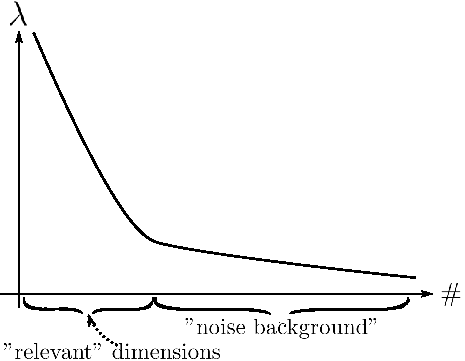
\includegraphics[width=8cm]{section2_fig4}  
  \caption{scree plots (ordering of eigenvalues by size):}
  \label{fig:screePlot}
\end{figure}

\paragraph{Comments:}
\begin{itemize}
\item variance is a scale sensitive measure (e.g.\ using centimeters instead
  of millimeters along one dimension will change all PCs)
	\item max. variance criterion only makes sense if scales are 
		''comparable''
	\item still: PCA constructs uncorrelated features (independent of scale)
	\item PCA is often used for ''whitening'': scale variance along all
		directions to one
\end{itemize}

% -----------------------------------------------------------------------------

\newpage 						% for visual reasons
\subsection{Hebbian Learning for Linear Neurons}
\begin{figure}[h]
  \centering
\[ \begin{array}{ll}
	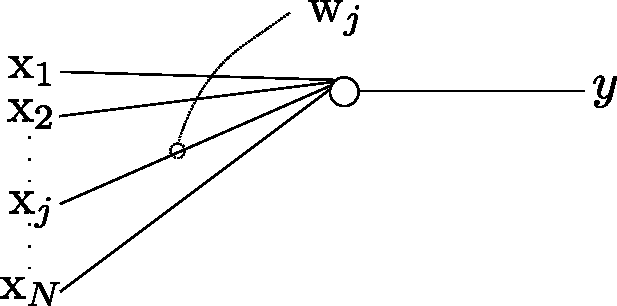
\includegraphics[width=6cm]{section2_fig5}
	& y = \vec{w}^T \vec{x}
\end{array} \]
  \caption{Linear connectionist neuron}
  \label{fig:linearConnectionistNeuron}
\end{figure}
observations: $\vec{x}^{(\alpha)}, \alpha = 1, \ldots, p, \vec{x}^{(\alpha)} \in \mathbb{R}^N$

\begin{algorithm}[h]
  \DontPrintSemicolon
  initialization of weights (e.g.\ to small numbers)\;
  choose learning rate $\varepsilon$\;
  \Begin(loop){
    Choose an observation  $\vec{x}^{(\alpha)}$\;
    Change weights according to:\;
    \begin{equation}
      \underbrace{ \Delta \mathrm{w}_j = \varepsilon 
        y_{ \big( \vec{x}^{(\alpha)}; \vec{w} \big) }
        \vec{x}^{(\alpha)} }_{
        \substack{\text{weights increase (decrease) if input}\\
          \text{and output are correlated (anticorrelated)}}}
    \end{equation}    
  }
  \label{alg:HebbianLearning}
  \caption{Hebbian (correlation-based) learning for linear neurons}
\end{algorithm}

\paragraph{Proposition:} Applied to linear neurons, Hebbs rule extracts the PC with the largest Eigenvalue.

\paragraph{Proof:}
small learning steps $\leadsto$ average over all patterns
\begin{equation}
	\begin{array}{ll}
		\Delta \mathrm{w}_j 
		& \approx \frac{\varepsilon}{p} \sum\limits_{\alpha = 1}^p 
			y_{\big( \vec{x}^{(\alpha)};
			\vec{w} \big) } \mathrm{x}_j^{(\alpha)} \\\\
		& = \frac{\varepsilon}{p} \sum\limits_{\alpha = 1}^p
			\sum\limits_{k = 1}^N \mathrm{w}_k
			\mathrm{x}_k^{(\alpha)} \mathrm{x}_j^{(\alpha)} \\\\
		& = \varepsilon \sum\limits_{k = 1}^N \mathrm{w}_k C_{kj}
	\end{array}
\end{equation}
\begin{equation}
	\Delta \vec{w} = \varepsilon \vec{C} \vec{w} \leadsto 
		\substack{ 	\text{''analysis'' of the} \\
				\text{covariance matrix} }
\end{equation}
transformation into the eigenbasis of $\vec{C}$
\\\\
let: $\lambda_1 > \lambda_2 > \ldots > \lambda_N \leftarrow$ eigenvalues
\begin{equation}
	\vec{w} = a_1 \vec{e}_1 + a_2 \vec{e}_2 + \ldots + a_N \vec{e}_N 
		\leftarrow \text{ corresponding eigenvectors}
\end{equation}
then:
\begin{equation}
	\Delta a_j = \varepsilon \lambda_j a_j
\end{equation}

\begin{figure}[h]
  \centering
\includegraphics[width=10cm]{section2_fig6}  
  \caption{Learning via Ojas rule}
  \label{fig:learningOjasRule}
\end{figure}



\begin{itemize}
	\itr $|\vec{w}| \rightarrow \infty$
	\itr $\vec{e}_{\mathrm{w}} = \frac{\vec{w}}{|\vec{w}|}$ converges to
		$\vec{e}_1$ (eigenvector with the largest eigenvectors)
\end{itemize}

Note: in the Haykin book a proof for the more general stochastic algorithm can be 
found showing the generality of the statement.

\paragraph{Neurobiological implications} 
\begin{itemize}
\item receptive fields and coding
\item adaptive tracking of the direction of largest variance: ''on-line'' PCA
\end{itemize}
%
\emph{Problem:} $\|w\| \to \infty$ \ra requires some form of normalization
\\\\
\emph{Solution:} Normalization via Oja's rule
\begin{equation}
	\Delta \mathrm{w}_j = \varepsilon y_{ \big( \vec{x}^{(\alpha)}; \vec{w}
		\big) } \bigg\{ 
			\underbrace{ \mathrm{x}_j^{(\alpha)} }_{
				\substack{	\text{Hebbian} \\
						\text{learning} }}
			- \underbrace{ y_{ \big( \vec{x}^{(\alpha)}; \vec{w}
				\big) } \mathrm{w}_j }_{ 
				\substack{	\text{decay} \\
						\text{term} }}
			\bigg\}
\end{equation}
Oja's rule converges to the unit vector which points into the direction of the
largest variance 
\\\\
{\it proof: supplementary material}

\paragraph{Hebbian PCA (generalized Hebbian algorithm):}
\begin{center}
		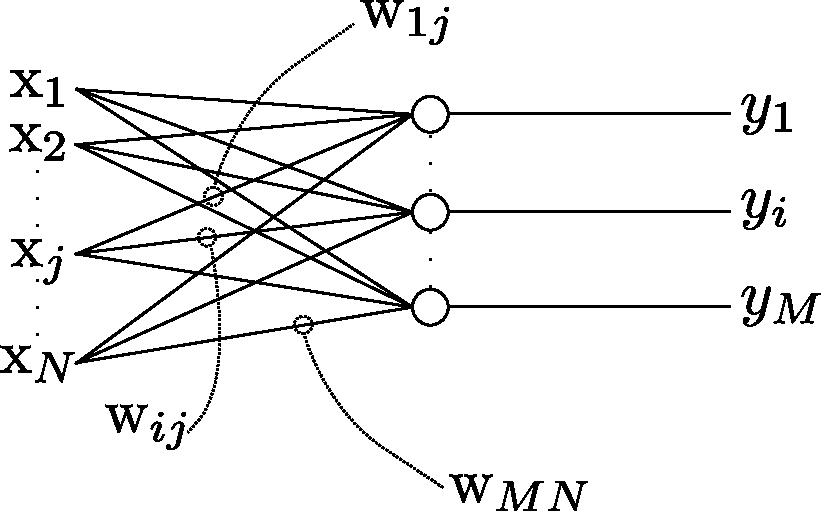
\includegraphics[width=6cm]{section2_fig5_b}
\end{center}
	$\text{M linear neurons: } y_i = \vec{w}_i^T \vec{x} = \sum_{j=1}^{N} \mathrm{w}_{ij} \mathrm{x}_j $, $i=1, \dots, M$\\
	observations: $\vec{x}^{(\alpha)},\quad \alpha = 1, \ldots, p,\quad \vec{x}^{(\alpha)} \in \mathbb{R}^N$ \\ 
	\vspace{5mm}
	The (feedforward) neural network extracts the $M$ PCs with the largest eigenvalues\\
	\begin{itemize}
		\itl online-PCA for data with time-varying statistics
	\end{itemize} 

\paragraph{Extended learning (Sanger's rule)}
\begin{equation*}
			\Delta \mathrm{w}_{ij} = \varepsilon y_i \bigg\{ \underbrace{\mathrm{x}_j}_{\text{Hebbian rule}} - \underbrace{\sum_{k=1}^{i} \mathrm{w}_{kj} y_k}_{\substack{\sum_{k=1}^{i-1} \mathrm{w}_{kj} y_k  \text{ is added to Oja's rule}}} \bigg\}
		\end{equation*}

\begin{itemize}
		\itl weights converge to the $M$ eigenvectors with the largest eigenvalues \\ \vspace{0.2cm}
\begin{tabular}{ccc}
			$\vec{w}_1$ & $\rightarrow$ & $\vec{e}_1$ \\ 
			$\vec{w}_2$ & $\rightarrow$ & $\vec{e}_2$ \\ 
						& $\vdots$ &  \\ 
			$\vec{w}_M$ & $\rightarrow$ & $\vec{e}_M$  
\end{tabular}
		\vspace{0.2cm}
		\itl $y_i = \vec{e}_i^T \vec{x} =: a_i$ after learning
\end{itemize}

\paragraph{Learning: Oja's rule \& Gram-Schmidt orthonormalization}\mbox{}\\
	Sanger's rule: $\Delta \mathrm{w}_{ij} = \varepsilon y_i \bigg\{ \mathrm{x}_j - \sum_{k=1}^{i} \mathrm{w}_{kj} y_k \bigg\}$
	\begin{itemize}
		\item Define $\hat{\mathrm{x}}_j^{(i)} := \mathrm{x}_j - \sum_{k=1}^{i-1} \mathrm{w}_{kj} y_k$
		\item Then $\Delta \mathrm{w}_{ij} = \varepsilon y_i \left\{ \hat{\mathrm{x}}_j^{(i)} - y_j \mathrm{w}_{ij} \right\} 		  					\longrightarrow$ Oja's rule with modified input
	\end{itemize}
	
\textbf{Case $i=1$:}:\\
\begin{tabular}{lll}
			$\hat{\mathrm{x}}_j^{(1)} = \mathrm{x}_j$ & $\leadsto$ & original form of Oja's rule \\
								                      & $\leadsto$ & $\vec{w}_1$ converges to eigenvector $\pm \vec{e}_1$
\end{tabular}\\
\vspace{0.3cm}
\begin{wrapfigure}{r}{0.5\textwidth}
  \begin{center}
    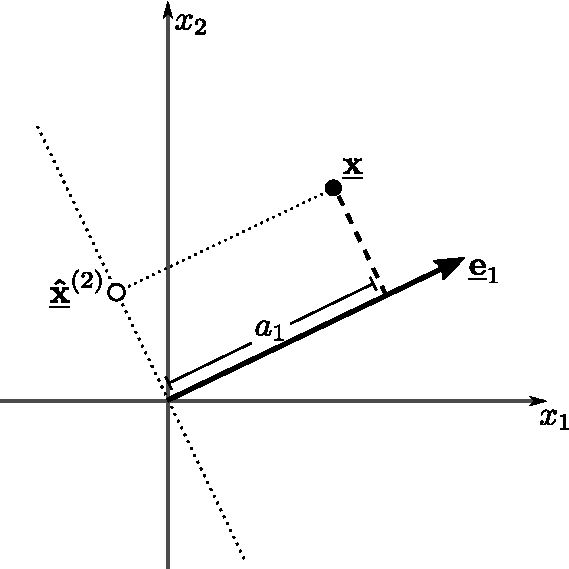
\includegraphics[width=0.4\textwidth]{section1_fig7}
  \end{center}
  \caption{novelty orthonormalization}
\end{wrapfigure}
\textbf{Case $i=2$:}\\
		$\hat{\mathrm{x}}_j^{(2)} = \mathrm{x}_j - \mathrm{w}_{1j} y_1$ \\
		$\vec{w}_1 = \vec{e}_1 \rightarrow y_1 = \vec{x}^T \vec{e}_1 =: a_1$ \\ \& $\hat{\mathrm{x}}_j^{(2)} = \mathrm{x}_j - \left( \vec{e}_1 \right)_j a_1$\\
\begin{itemize}
	\itr $\hat{\vec{x}}^{(2)}$ is the projection of $\vec{x}$ onto subspace orthogonal to $\vec{e}_1$:
	\begin{itemize}
	\itr $\vec{w}_2$ converges to $\pm \vec{e}_2$ by Oja's rule since $\vec{e}_2$ is the direction of largest variance in that subspace
	\end{itemize}
\end{itemize}
\vspace{0.7cm}
\textbf{Case $i=3$:}\\
$\hat{\mathrm{x}}_j^{(3)} = \mathrm{x}_j - \mathrm{w}_{1j} y_1 - \mathrm{w}_{2j} y_2$ \\ 
$$\vec{w}_1 = \vec{e}_1 \hspace{0.1cm} \& \hspace{0.1cm} \vec{w}_2 = \vec{e}_2 \rightarrow y_1 = a_1, \hspace{0.2cm} y_2 = \vec{x}^T \hspace{0.2cm} \vec{e}_2 =: a_2\\ 
\hspace{0.1cm} \& \hspace{0.1cm}\hat{\mathrm{x}}_j^{(3)} = \mathrm{x}_j - a_1 \left( \vec{e}_1 \right)_j - a_2 \left( \vec{e}_2 \right)_j$$
\begin{itemize}
\itr $\hat{\vec{x}}^{(3)}$ is the projection of $\vec{x}$ onto subspace orthogonal to $\operatorname{span}\left\{ \vec{e}_1, \vec{e}_2 \right\}$
\itr $\vec{w}_3$ converges to $\pm \vec{e}_3$ by Oja's rule\\
\end{itemize}
\vspace{0.1cm}
\textbf{Case $i=M$:}\\
$\hat{\mathrm{x}}_j^{(M)} = \mathrm{x}_j - \sum_{k=1}^{M-1} \mathrm{w}_{kj} y_k$ \\
$\vec{w}_k = \vec{e}_k \text{ for }k=1,\dots, M-1 \rightarrow y_k = \vec{x}^T \vec{e}_k =: a_k$ \\ 
\& $\hat{\mathrm{x}}_j^{(M)} = \mathrm{x}_j - \sum_{k=1}^{M-1} a_k \left( \vec{e}_k \right)_j$ 

\begin{itemize}
\itr $\hat{\vec{x}}^{(M)}$ is the proj. of $\vec{x}$ onto subspace orthogonal to $\operatorname{span}\left\{ \vec{e}_1, \hdots, \vec{e}_{M-1} \right\}$ 
\itr $\vec{w}_M$ converges to $\pm \vec{e}_M$ by Oja's rule
\end{itemize}

\paragraph{Summary of Hebbian learning: }\mbox{}\\
\textbf{I. Hebbian learning without constraint}\\
		\begin{equation*}
			\underbrace{\Delta \vec{w} = \varepsilon y \vec{x}}_{\text{Hebb's rule}} \leadsto \lim\limits_{t \rightarrow \infty} \vec{w} || \vec{e}_1 \text{ (orthogonal)}
		\end{equation*}
$\leadsto$ weights converge to direction of largest variance in the data\\
$\leadsto$ but: $|\vec{w}| \rightarrow \infty$ for $t \rightarrow \infty$

\textbf{II. Hebbian learning with normalization}\\
		\begin{equation*}
			\underbrace{\Delta \vec{w} = \varepsilon y \left( \vec{x} - y \vec{w} \right)}_{\text{Oja's rule}} \leadsto \lim\limits_{t \rightarrow \infty} \vec{w} \in \left\{ +\vec{e}_1, -\vec{e}_1 \right\}
		\end{equation*}
$\leadsto$ weights remain finite: $|\vec{w}| = 1$

\textbf{III. Hebbian PCA with $M$ neurons and normalization}\\
		\begin{equation*}
			\underbrace{\Delta \mathrm{w}_{ij} = \varepsilon y_i \left\{ \mathrm{x}_j - \sum_{k=1}^{i} \mathrm{w}_{kj} y_k \right\} }_{\text{Sanger's rule}} \leadsto \lim\limits_{t \rightarrow \infty} \vec{w}_i \in \left\{ +\vec{e}_i, -\vec{e}_i \right\}, i=1, \hdots, M
		\end{equation*}
		$\leadsto$ combination of Oja's rule \& Gram-Schmidt-orthonormalization




% -----------------------------------------------------------------------------

\newpage 						% for visual reasons
\subsection{Kernel Principal Component Analysis}
Kernel PCA extends the linear dimensionality reduction approach of PCA to extract nonlinear structure. 
% -----------------------------------------------------------------------------
\subsubsection{Non-linear Manifolds}
\begin{figure}[h]
  \centering
\includegraphics[width=8cm]{section2_fig7}  
  \caption{Example of a nonlinear dependency}
  \label{fig:nonlinearDependency}
\end{figure}
%
Consider the data represented in the original space:
\begin{itemize}
  \item standard PCA: two directions with high variance
  \item ''interesting'' feature is a non-linear combination of
    elementary features \itl this dependency is not properly extracted
    by standard PCA
\end{itemize}

\begin{figure}[h]
  \centering
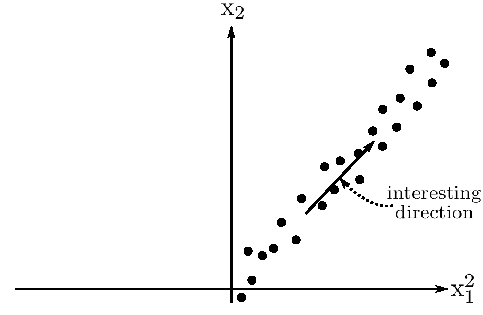
\includegraphics[width=8cm]{section2_fig8}  
  \caption{Nonlinear dependency becomes linear in transformed space}
  \label{fig:transformedDependency}
\end{figure}


Idea: analyse data in \emph{transformed} (feature) space:
\begin{itemize}
	\itl standard PCA: one direction of high variance
	\itl ''interesting'' feature will be discovered
\end{itemize}
\textbf{Agenda:} non-linear preprocessing, then application of a
standard linear method $\Rightarrow$ non-linear analysis method,
i.e.\ given a set of observations: $\vec{x}^{(\alpha)}, \alpha = 1,
\ldots, p; \vec{x}^{(\alpha)} \in \mathbb{R}^N$
\begin{enumerate}[(1)]
\item transformation into an ''appropriate'' feature space
\begin{equation}
	\vec{\phi}: \vec{x} \rightarrow \vec{\phi}_{(\vec{x})}
\end{equation}
\item apply \emph{linear} analysis method on $\vec{\phi}_{(\vec{x})}$
\end{enumerate}
\textbf{Problem:} Some feature spaces may be extremely high-dimensional

\begin{figure}[h]
  \centering
\includegraphics[width=3cm]{section2_fig9}  
  \caption{Pixel image as a high dimensional patterns}
  \label{fig:pixelImage}
\end{figure}


\begin{itemize}
  \itl interesting structure is hidden in correlations between pixel 
  values
  \itl 'interesting'' feature space: space spanned by all 
  $d^{\mathrm{th}}$-order monomials
  \begin{equation}
    \text{e.g. } d = 2: 
    \mathrm{x}_1^2, \mathrm{x}_1 \mathrm{x}_2, 
    \mathrm{x}_2^2, \mathrm{x}_1 \mathrm{x}_3, 
    \mathrm{x}_2 \mathrm{x}_3, \mathrm{x}_3^2, \ldots
  \end{equation}
  \itl number of dimensions
  \begin{equation}
    \frac{ (N+d-1)! }{ d!(N-1)! } 
    = O_{ \big( N^d \big) }
  \end{equation}
\end{itemize}
Are there methods which work in the original space $\mathbb{R}^N$? \\
Yes! Use the kernel trick ({\it see also MI I, chapter 2.2.4}).

% -----------------------------------------------------------------------------
\subsubsection{Reformulation of PCA using only Scalar Products}
Observations: $\vec{x}^{(\alpha)}, \alpha = 1, \ldots, p; \vec{x}^{(\alpha)} \in \mathbb{R}^N$
\\\\
Simplifying assumptions:
\begin{equation}
	\frac{1}{p} \sum\limits_{\alpha = 1}^p \vec{x}^{(\alpha)} = \vec{0}
		\leadsto \text{ zero mean data}
\end{equation}
Correlation matrix $\vec{C}$:
\begin{equation}
	C_{ij} = \frac{1}{p} \sum\limits_{\alpha = 1}^p \mathrm{x}_i^{(\alpha)}
		\mathrm{x}_j^{(\alpha)} 
		\Rightarrow \vec{C} = \frac{1}{p} \sum\limits_{\alpha = 1}^p
			\vec{x}^{(\alpha)} \Big( \vec{x}^{(\alpha)} \Big)^T
\end{equation}
PCA requires a solution of the eigenvalue problem:
\begin{equation}
	\vec{C} \vec{e}_k = \lambda_k \vec{e}_k
\end{equation}
Expansion of the eigenvectors into data points (linear combination, not necessarily unique):
\begin{equation}
	\underbrace{ \vec{e}_k = \sum\limits_{\beta = 1}^p a_k^{(\beta)} 
		\vec{x}^{(\beta)}
	}_{ \substack{	\text{always possible, because principal 
					components}\\
				\text{lie in the subspace of the data} } }
\end{equation}
Insertion into the eigenvalue equation leads to:
\begin{equation}
	\frac{1}{p} \sum\limits_{\alpha, \beta = 1}^p a_k^{(\beta)}
	\bigg[ \Big( \vec{x}^{(\alpha)} \Big)^T \vec{x}^{(\beta)} \bigg]
	\vec{x}^{(\alpha)} = \lambda_k \sum\limits_{\beta = 1}^p
	a_k^{(\beta)} \vec{x}^{(\beta)}
\end{equation}
%Projections onto the directions given by data points $\Big( \vec{x}^{(\gamma)} \Big)^T$:
Multiplying with data points $\Big( \vec{x}^{(\gamma)} \Big)^T$, $\gamma = 1,\dots,p$:
\begin{equation}
	\frac{1}{p} \sum\limits_{\alpha, \beta = 1}^p a_k^{(\beta)}
	\bigg[ \Big( \vec{x}^{(\alpha)} \Big)^T \vec{x}^{(\beta)} \bigg]
	\bigg[ \Big( \vec{x}^{(\gamma)} \Big)^T \vec{x}^{(\alpha)} \bigg]
	= \lambda_k \sum\limits_{\beta = 1}^p a_k^{(\beta)} 
	\bigg[ \Big( \vec{x}^{(\gamma)} \Big)^T \vec{x}^{(\beta)} \bigg]
\end{equation}
Formulation of the eigenvalue problem in terms of scalar products:
\begin{equation}
	K_{\alpha \beta} \coloneqq \Big( \vec{x}^{(\alpha)} \Big)^T 
		\vec{x}^{(\beta)}
\end{equation}
in matrix notation (generalized eigenvalue problem):
\begin{equation}
	\vec{K}^2 \vec{a}_k = p \lambda_k \vec{K} \vec{a}_k
\end{equation}
\textbf{Remark:} $\vec{K}$ is a positive semidefinite matrix! Why? Because
for an arbitrary vector $\vec{y}$:
\begin{equation}
	\begin{array}{ll}
	\vec{y}^T \vec{K} \vec{y} 
	& = \sum\limits_{\alpha, \beta = 1}^p
		y^{(\alpha)} \Big( \vec{x}^{(\alpha)} \Big)^T
		\vec{x}^{(\beta)} y^{(\beta)} \\\\
	& = \Bigg( \sum\limits_{\alpha = 1}^p y^{(\alpha)} \vec{x}^{(\alpha)}
		\Bigg)^2 \\\\
	& \geq 0
	\end{array}
\end{equation}

Positive semidefiniteness of $\vec{K}$
means,
it has only non-negative eigenvalues (but potentially 0) 
\ra
% can be inverted \ra multiply by $K^{-1}$ from the left. \ra 
solutions
of the following transformed (standard eigenvalue) problem differ only by components corresponding to
% orthogonal to the
uninteresting directions with zero eigenvalues
% solution space 
(see e.g.\ \cite{Bishop2006}).
\\\\
Transformed eigenvalue problem:
\begin{equation}
	\fbox{$ \vec{K} \vec{a}_k = p \lambda_k \vec{a}_k $}
\end{equation}
\[ \begin{array}{ll}
	\vec{K}: & \text{matrix of scalar products between data points} \\\\
	\lambda_k: & \text{variance along principal component } \vec{a}_k \\\\
	\vec{a}_k: & \text{principal component, represented in the - may be 
		autocomplete -} \\
	&	\text{basis } \Big\{ \vec{x}^{(\alpha)} \Big\}, 
		\alpha = 1, \ldots, p
\end{array} \]
Normalization of principal components
\begin{equation}
	\begin{array}{ll}
		\vec{e}_k^2 
		& = \sum\limits_{\alpha, \beta = 1}^p a_k^{(\alpha)} 
			\Big( \vec{x}^{(\alpha)} \Big)^T \vec{x}^{(\beta)}
			a_k^{(\beta)} \\\\
		& = \vec{a}_k^T \vec{K} \vec{a}_k  \\\\
		& = \lambda_k \vec{a}_k^2 p\\\\
		& \eqexcl 1
	\end{array}
\end{equation}
\begin{equation}
	\fbox{$ \vec{a}_k^{\mathrm{norm.}} = 
			\frac{1}{\sqrt{p} \sqrt{\lambda_k} |\vec{a_k}|} 
			\vec{a}_k $}
\end{equation}
Projection $u_k$ of a new data vector $\vec{x}$ onto the principal components
\begin{equation}
	\begin{array}{ll}
	u_k
	& = \vec{e}_k^T \cdot \vec{x} \\\\
	& = \sum\limits_{\beta = 1}^p a_k^{(\beta)} 
		\underbrace{ \bigg[ \Big( \vec{x}^{(\beta)} \Big)^T 
				\cdot \vec{x} \bigg] }_{
					\text{scalar product} }
	\end{array}
\end{equation}
\textbf{Note:} This formulation of PCA is exclusively in terms of scalar products
\\\\
% -----------------------------------------------------------------------------

\subsubsection{The Kernel Trick}
\textbf{Idea:} perform PCA in a suitable feature space
\begin{equation}
	\vec{\phi}: \vec{x} \xrightarrow{\text{ {\tiny non-linear 
		transformation}}} \vec{\phi}_{(\vec{x})}
\end{equation}
\textbf{Kernel trick:}
\begin{itemize}
	\itR avoid direct transformation $\vec{\phi}$
	\itR replace all scalar products by ''kernel functions''
		\begin{equation}
			\vec{\phi}_{(\vec{x})}^T
			\vec{\phi}_{(\vec{x}')} \longleftrightarrow 
			k_{(\vec{x}, \vec{x}')}
		\end{equation}
\end{itemize}

\paragraph{Mercer's theorem:} 
every positive definite kernel $k$ corresponds to a scalar product in 
some metric feature space\footnote{for details see MI I, chapt. 2.2.4} 
\\\\
{\bf Typical kernel functions}
\[ \begin{array}{ll}
	k_{(\vec{x},\vec{x}')} = \big( \vec{x}^T \vec{x}' + 1 \big)^d
	& \substack{	\text{polynomial kernel of degree } d \\
			\text{{\it image processing (pixel correlation)}} } \\\\
	k_{(\vec{x},\vec{x}')} = \exp \bigg\{ -\frac{ \big( \vec{x} - \vec{x}' 
					\big)^2 }{ 2 \sigma^2 } \bigg\}
	& \substack{ 	\text{RBF-kernel with range } \sigma \\
			\text{{\it infinite dimensional feature space}} } \\\\
	k_{(\vec{x},\vec{x}')} = \tanh \big\{ K \vec{x}^T \vec{x}' + \theta
					\big\}
	& \substack{ 	\text{neural network kernel with parameters } K 
				\text{ and } \theta \\
			\text{{\it not necessarily positive definite}} } \\\\
	k_{(\vec{x},\vec{x}')} = \frac{1}{ |\vec{x} - \vec{x}' + \varepsilon
						|^N }
	& \substack{	\text{Plummer kernel with parameter } \varepsilon \\
			\text{{\it scale invariant kernel}} }
\end{array} \]
\textbf{Note:} no need to explicitly project into feature space -- if
an algorithm can be formulated solely in terms of scalar products, a
non-linear version of it can be derived via this approach. 
\begin{itemize}
	\itl {\it cf. support vector machines (MI I)}
	\itl Fisher discriminant analysis, Canonical Correlation Analysis
	\itl K-means clustering \& self-organizing maps (MI II)
\end{itemize}

\noindent \textbf{Problem: } derivation assumes zero mean -- but
normalization to zero mean in original space does not guarantee normalization in
feature space
\begin{equation}
        \frac{1}{p} \sum\limits_{\alpha = 1}^p \vec{x}^{(\alpha)} \eqexcl 0
        \nrightarrow \frac{1}{p} \sum\limits_{\alpha = 1}^p 
                \vec{\phi}_{\big( \vec{x}^{(\alpha)} \big)} = \vec{0}
\end{equation}
\textbf{Solution:} calculation of ''centered'' kernel matrix elements 
\\\\
data points $\vec{x}^{(\alpha)}$: ''training'' data: $\alpha \in \{1, \ldots, p\}$; new (test) data: $\alpha > p$
\begin{equation}
        \underbrace{ \vec{\phi}_{\big( \vec{x}^{(\alpha)} \big)} }_{
                \substack{      \text{''centered''} \\
                                \text{feature vectors}} }
        = \widetilde{\vec{\phi}}_{\big( \vec{x}^{(\alpha)} \big)}
                - \frac{1}{p} \sum\limits_{\gamma = 1}^p 
                \underbrace{ \widetilde{\vec{\phi}}_{\big( \vec{x}^{(\gamma)} 
                                \big)} }_{
                        \substack{      \text{uncentered} \\
                                        \text{feature vectors}} }
\end{equation}
\begin{equation}
        \begin{array}{lll}
        K_{\alpha \beta}
        & = & \vec{\phi}_{\big( \vec{x}^{(\alpha)} \big)}^T
                \cdot \vec{\phi}_{\big( \vec{x}^{(\beta)} \big)}
                \\\\
        & = & \bigg( \widetilde{\vec{\phi}}_{\big( \vec{x}^{(\alpha)} \big)}^T
                - \frac{1}{p} \sum\limits_{\gamma = 1}^p 
                \widetilde{\vec{\phi}}_{\big( \vec{x}^{(\gamma)} \big)}^T
                \bigg) \bigg(\widetilde{\vec{\phi}}_{\big( \vec{x}^{(\beta)} 
                \big)} - \frac{1}{p} \sum\limits_{\delta = 1}^p 
                \widetilde{\vec{\phi}}_{\big( \vec{x}^{(\delta)} \big)} \bigg)
                \\\\
        & = & \widetilde{\vec{\phi}}_{\big( \vec{x}^{(\alpha)} \big)}^T
                \widetilde{\vec{\phi}}_{\big( \vec{x}^{(\beta)} \big)}
                - \frac{1}{p} \sum\limits_{\gamma = 1}^p 
                \widetilde{\vec{\phi}}_{\big( \vec{x}^{(\gamma)} \big)}^T
                \widetilde{\vec{\phi}}_{\big( \vec{x}^{(\beta)} \big)}
                \\\\
        && - \frac{1}{p} \sum\limits_{\delta = 1}^p 
                \widetilde{\vec{\phi}}_{\big( \vec{x}^{(\alpha)} \big)}^T
                \widetilde{\vec{\phi}}_{\big( \vec{x}^{(\delta)} \big)}
                + \frac{1}{p^2} \sum\limits_{\delta = 1}^p 
                \widetilde{\vec{\phi}}_{\big( \vec{x}^{(\gamma)} \big)}^T
                \widetilde{\vec{\phi}}_{\big( \vec{x}^{(\delta)} \big)}
                \\\\
        & = & \widetilde{K}_{\alpha \beta} - \frac{1}{p} 
                \sum\limits_{\gamma = 1}^p \widetilde{K}_{\gamma \beta}
                -\frac{1}{p} \sum\limits_{\gamma = 1}^p 
                \widetilde{K}_{\alpha \gamma} + \frac{1}{p^2} 
                \sum\limits_{\gamma, \delta} \widetilde{K}_{\gamma \delta}
        \end{array}
\end{equation}



% -----------------------------------------------------------------------------

\subsubsection{Summary of the Kernel-PCA Method}
\begin{enumerate}[(1)]
\item calculate the un-normalized kernel matrix $\widetilde{\vec{K}}$
\begin{equation}
	\widetilde{K}_{\alpha \beta} = \underbrace{ k_{\big( \vec{x}^{(\alpha)},
			\vec{x}^{(\beta)} \big)} }_{
				\substack{ 	\text{kernel} \\
						\text{function}} }
\end{equation}
\item normalize to zero mean
\begin{equation}
	K_{\alpha \beta} = \widetilde{K}_{\alpha \beta} - \frac{1}{p} 
		\sum\limits_{\gamma = 1}^p \widetilde{K}_{\gamma \beta}
		-\frac{1}{p} \sum\limits_{\gamma = 1}^p 
		\widetilde{K}_{\alpha \gamma} + \frac{1}{p^2} 
		\sum\limits_{\gamma, \delta} \widetilde{K}_{\gamma \delta}
\end{equation}
\item solve the eigenvalue problem
\begin{equation}
	\vec{K} \widetilde{\vec{a}}_k = p \lambda_k \widetilde{\vec{a}}_k
\end{equation}
\item normalize eigenvectors to unit length (in feature space)
\begin{equation}
	\vec{a}_k = \frac{1}{\sqrt{p \lambda_k} \, ||\widetilde{\vec{a}}_k||} 
			\widetilde{\vec{a}}_k
\end{equation}
\item calculate projections of data points $\vec{x}^{(\alpha)}$ onto eigenvectors
\begin{equation}
	u_k(\vec{x}^{(\alpha)}) = \sum\limits_{\beta = 1}^p a_k^{(\beta)} 
		K_{\beta \alpha} \leftarrow 
			\substack{	\text{use normalized} \\
					\text{matrix element!}}
\end{equation}
\end{enumerate}

More generally, for arbitrary $\vec{x}$ the projection is computed as:

\begin{align*}
	u_{k}\left (\vec{x} \right ) 
	= & \sum\limits_{\beta = 1}^p a_k^{(\beta)} \vec{\phi}_{\left(\vec{x}^{(\beta)}\right)}^T 
	    \vec{\phi}_{(\vec{x})}	\qquad \leftarrow \text{\scriptsize centered feature vectors} \\
	=  & \sum\limits_{\beta = 1}^p a_k^{(\beta)} 
	    \Big ( \Big [ \widetilde{\vec{\phi}}_{\left(\vec{x}^{(\beta)}\right)}
			  - \frac{1}{p} \sum\limits_{\gamma=1}^p 
				  \widetilde{\vec{\phi}}_{\left(\vec{x}^{(\gamma)}\right)} \Big ]^T 
		   \Big [ \widetilde{\vec{\phi}}_{\left(\vec{x}\right)} 
			  - \frac{1}{p} \sum\limits_{\delta=1}^p 
			      \widetilde{\vec{\phi}}_{\left(\vec{x}^{(\delta)}\right)} \Big ]
	    \Big ) \\
	= &  \sum\limits_{\beta = 1}^p a_k^{(\beta)} 
	    \Big (
		k(\vec{x}^{(\beta)}, \vec{x})
		- \frac{1}{p} \sum\limits_{\delta=1}^p \widetilde K_{\beta \delta} 
		- \frac{1}{p} \sum\limits_{\gamma=1}^p k(\vec{x}^{(\gamma)}, \vec{x})
		+ \frac{1}{p^2} \sum\limits_{\gamma,\delta=1}^p \widetilde K_{\gamma \delta}
	    \Big )
\end{align*}


\paragraph{Comments:}
\begin{itemize}
\item kernel-PCA $\corresponds$ PCA in feature space
  \begin{itemize}
    \itr ''principal components'' are uncorrelated
    \itr $\lambda_k$: variance of the data along principal component
    $k$ ( in feature space)
    \itr mean-squared approximation error (in feature space) in representing the 
    observations by components with largest eigenvalues
    is minimal
  \end{itemize}
\item for KPCA, number of principal components can exceed number of
  dimensions in the original space
  \item reconstruction is harder as in linear PCA: no explicit data space representation of the 
  principal component subspace
  \begin{itemize}
   \item typically only projection coefficients $u_k(\vec{x})$ are used
   \item data space is mapped to low-dim. manifold in feature space
   \item for general feature vectors: no pre-image in data space
   \item but: approximative pre-images can be computed (application: denoising)
  \end{itemize}
  \item Kernel PCA can be used for feature extraction, e.g., to solve classification problems in feature space
  \item Optimal kernel parameters ($\sigma$, $d$, etc.) depend on data \& task (selection via cross-validation possible for classification tasks but in general no measure-of-goodness of the PC projections available)
  \item Custom kernels can be used (any positive definite kernel matrix)
\item expansion of principal components into data points is 
  \underline{not} sparse
    $\leadsto$ high computational burden when calculating projections
    \\\\
    \emph{possible solution:} approximate principal components using expansions with less data
    vectors $q < p$:
    \begin{equation*}
      \begin{array}{ll}
        \vec{e}_k = \sum\limits_{\beta = 1}^p a_k^{(\beta)}
        \vec{\phi}_{\big( \vec{x}^{(\beta)} \big)}
        & \text{principal (normalized) components } k
        \\\\
        \widehat{\vec{e}}_k = \sum\limits_{\gamma = 1}^q
        \widehat{a}_k^{(\gamma)} 
        \vec{\phi}_{ \underbrace{ \big( 
            \vec{z}^{(\gamma)} \big) }_{
%             \substack{ 	\text{new data} \\
%               \text{pt. order, } \\ }
          }}
        & \text{approximation by $q$ data points \big(in new order, $\vec z^{(\gamma)} = \vec x^{(i_\gamma)}$\big)}
      \end{array}
    \end{equation*}
    quadratic error  $\varphi$:
    \begin{equation*}
      \begin{array}{ll}
        \varphi
        & = \big( \vec{e}_k - \widehat{\vec{e}}_k \big)^2
        \\\\
        & = \underbrace{ |\vec{e}_k|^2 }_{= 1} 
        + | \widehat{\vec{e}}_k |^2 - 2\vec{e}_k^T
        \widehat{\vec{e}}_k
        \\\\
        & = 1 + \sum\limits_{\gamma, \delta = 1}^q 
        \widehat{a}_k^{(\gamma)} 
        \widehat{a}_k^{(\delta)} k_{\big( 
          \vec{z}^{(\gamma)}, \vec{z}^{(\delta)}
          \big)}
        -2 \sum\limits_{\beta = 1}^p 
        \sum\limits_{\gamma = 1}^q 
        a_k^{(\beta)} \widehat{a}_k^{(\gamma)}
        k_{\big( \vec{x}^{(\beta)}, \vec{z}^{(\gamma)}
          \big)}
      \end{array}
    \end{equation*}
    choose $\widehat{a}_k^{(\gamma)}$ and $\vec{z}^{(\gamma)}$ such
    that
    \begin{equation*}
      \varphi \eqexcl \min
    \end{equation*}
    e.g.\ using gradient-based methods

  \item kernel matrices may be very large
  \begin{itemize}
    \itr only eigenvectors to the largest eigenvalues are
    of interest
    \itr use specialized routines (\cite{PressEtAl2007} chapt. 11.5 - 11.7)
  \end{itemize}
  \slideref{toy example (Schölkopf et al., MPI Biol. Cybern.
    Technical Report 44, Fig. 2)}
\end{itemize}

\subsection{Novelty Filter}
Principal Components with smallest eigenvalues (e.g., $\vec e_N$):
\begin{center}
 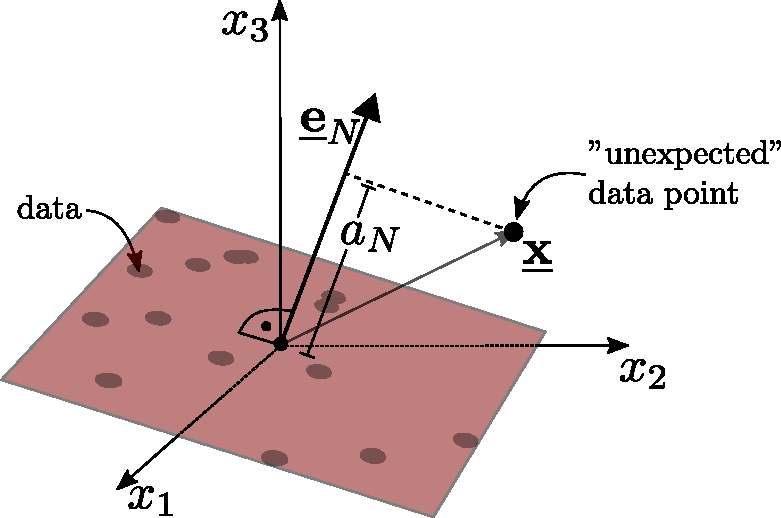
\includegraphics[width=6cm]{section1_fig6} 
\end{center}
%\pause
\begin{itemize}
        \itl outliers / data with novel features can be identified by projecting to last PCs
        \itl $y = \vec{e}_N^T \vec{x} =: a_N$ after learning $\leadsto$ projection onto smallest PC
        \itl large output for unexpected data $\rightarrow$ Novelty Filter
\end{itemize}

\paragraph{Novelty Filter: On-line Learning}
	\[ \begin{array}{ll}
	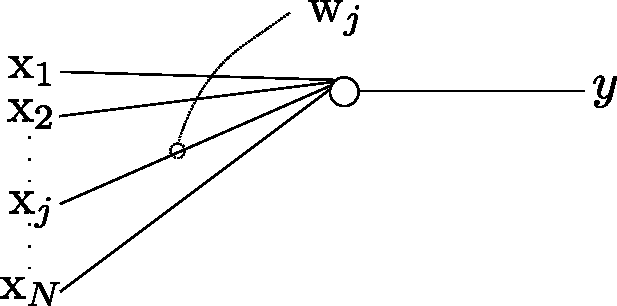
\includegraphics[width=5cm]{section2_fig5}
	& y = \vec{w}^T \vec{x}
	\end{array} \]
\textbf{Anti-Hebbian rule:} \\
\begin{equation}
				\Delta \mathrm{w}_j = \overbrace{-}^{\substack{	\text{''Anti''-} \\ \text{Hebbian} }} \varepsilon y^{(\alpha)} \mathrm{x}_j^{(\alpha)}
\end{equation}\\

Conjecture:\\ 
$\vec{w}$ converges to the direction of smallest eigenvector.\\
Proof:\\
Learning rule:
		\begin{equation}
		\Delta \mathrm{w}_j = - \varepsilon y^{(\alpha)} \mathrm{x}_j^{(\alpha)}
		\end{equation}
		Assume small learning steps $\rightarrow$ average over all patterns 
		\begin{equation}
			\Delta \mathrm{w}_j = - \frac{\varepsilon}{p} \sum_{\alpha = 1}^{p} y^{(\alpha)} \mathrm{x}_j^{(\alpha)} = - \frac{\varepsilon}{p} \sum_{\alpha = 1}^{p} \mathrm{x}_j^{(\alpha)} \sum_{k=1}^{N} \mathrm{x}_k^{(\alpha)} \mathrm{w}_k = - \varepsilon \sum_{k=1}^{N} C_{jk} \mathrm{w}_k 
		\end{equation}
		\begin{equation}
			\Delta \vec{w} = - \varepsilon \vec{C} \vec{w}
		\end{equation}

\begin{figure}[h]
\centering
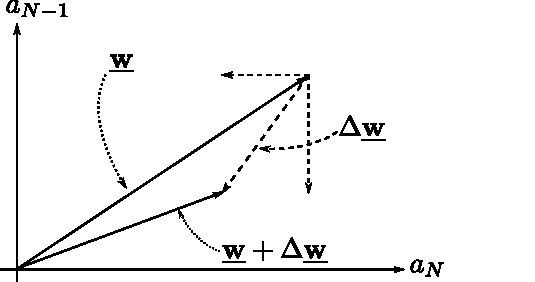
\includegraphics[width=7.5cm]{section2_fig6_a.pdf}
\end{figure}
Transformation into eigenbasis of covariance matrix:
\begin{align*}
			& \vec{w} = a_1 \vec{e}_1 + a_2 \vec{e}_2 + \dots + a_N \vec{e}_N\\
			& \Delta a_j = - \varepsilon \lambda_j a_j
s\end{align*}

\begin{itemize}
			\itl for $\lambda_j > 0: a_j \rightarrow 0$, constraints required
			\itl for $\lambda_j = 0: a_j$ remains unchanged
			\itl weights converge to the eigenvector with the smallest eigenvalue
\end{itemize}
\paragraph{Novelty Filter and linear regression}
\begin{center}
		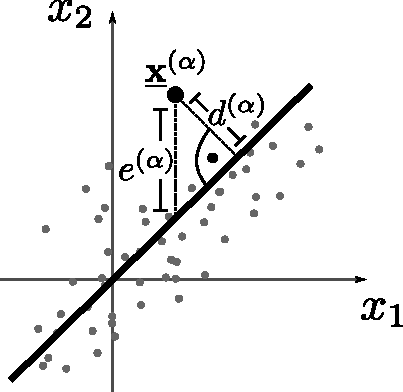
\includegraphics[width=3.6cm]{section2_fig6_b} \\
\end{center}
Ordinary least squares:\\
\begin{equation*}
		\frac{1}{p} \sum_{\alpha = 1}^{p} \left( e^{(\alpha)} \right)^2 \overset{!}{=} \text{min.}
\end{equation*}
\begin{itemize}
			\itl correct if data points are noisy along $x_2$-component only
			\itl wrong if data points are also noisy along $x_1$-component
\end{itemize}
total least squares:\\
\begin{equation*}
				\frac{1}{p} \sum_{\alpha =1}^{p} \left( d^{(\alpha)} \right)^2 \overset{!}{=} \text{min.}
\end{equation*}
tacit assumption: same variance noise \\
	centered data $\rightarrow \vec{w}^T\vec{x} = 0$ 

Cost function:
\begin{equation*}
		\mathbb{E}(\vec{w}) = \frac{1}{p} \sum_{\alpha =1}^{p} \left( d^{(\alpha)} \right)^2 \stackrel{!}{=} \min_{\vec{w}} \quad \text{s.t.} \abs{\vec{w}} = 1
\end{equation*}
\begin{equation*}
			\vec{w}^T \vec{C} \vec{w} \overset{!}{=} \min_{\vec{w}} \quad \text{s.t.} \abs{\vec{w}} = 1
\end{equation*}
\underline{solution}:\\
		$\vec{w}$ is the normalized eigenvector to the smallest eigenvalue of the covariance matrix.

\paragraph{Novelty Filter with normalization}
\begin{equation*}
		\Delta \vec{w} = - \varepsilon  \frac{y^{(\alpha)} \left\{ \vec{x}^{(\alpha)} - y^{(\alpha)} \vec{w} \right\}}{\abs{\vec{w} - \varepsilon y^{(\alpha)} \left\{ \vec{x}^{(\alpha)} - y^{(\alpha)} \vec{w} \right\}}}
\end{equation*}
Anti-Hebbian version of Oja's rule:\\
\begin{equation*}
			\Delta \mathrm{w}_j = - \varepsilon y^{(\alpha)} \Bigl\{ \overbrace{\mathrm{x}_j^{(\alpha)}}^{\substack{\text{Anti-Hebbian} \\ \text{learning}}} \underbrace{ - y^{(\alpha)} \mathrm{w}_j \Bigr\} + \varepsilon \Bigl\{ 1- \overbrace{\sum_{k=1}^{N} \mathrm{w}_k^2}^{=\abs{\vec{w}}^2} \Bigr\} \mathrm{w}_j}_{\text{normalization}}
\end{equation*}
\begin{itemize}
		\itl $\vec{w}$ converges to $\pm \vec{e}_N$
\end{itemize}

\paragraph{Feedforward network as a Novelty Filter}\mbox{}\\
Extension of the learning rule to N neurons:\\
\begin{equation*}
				\begin{aligned}
					\Delta \mathrm{w}_{ij} = 
					& - \varepsilon y_i^{(\alpha)} \Bigl\{ \mathrm{x}_j^{(\alpha)} - \overbrace{\sum_{k=1}^{i} \mathrm{w}_{kj} y_k^{(\alpha)}}^{-\sum_{k=1}^{i-1} \mathrm{w}_{kj} y_k^{(\alpha)} \text{is added}} \Bigr\} \\
					& + \varepsilon \Bigl\{ 1- \sum_{k=1}^{N} \mathrm{w}_{ik}^2 \Bigr\} \mathrm{w}_{ij}
				\end{aligned}
\end{equation*}
\begin{center}
\centering
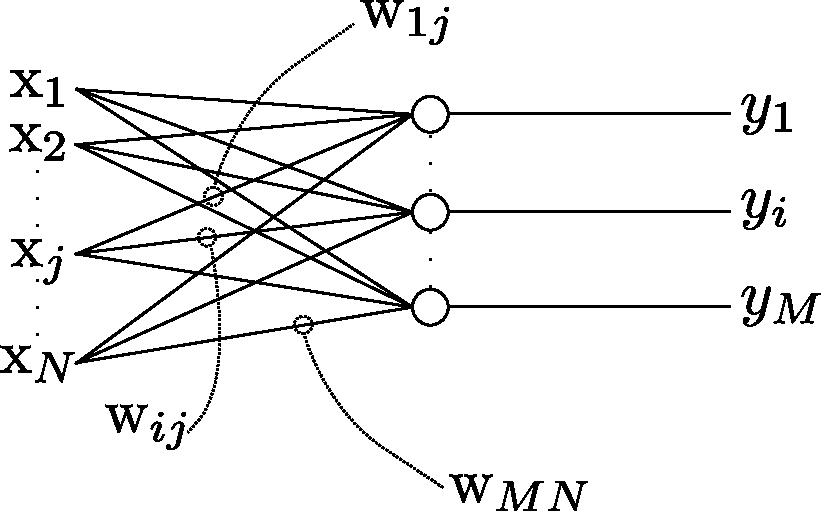
\includegraphics[width=0.5\textwidth]{section2_fig5_b}
\end{center}
\begin{tabular}{cll}
		$\leadsto$ result: & $\vec{w}_1 \rightarrow \vec{e}_N$ & (PC with smallest eigenvalue) \\ 
		& $\vec{w}_2 \rightarrow \vec{e}_{N-1}$ & $\vdots$ \\ 
		& $\vdots$ & $\vdots$ \\ 
		& $\vec{w}_M \rightarrow \vec{e}_{N-M+1}$ & (PC with largest eigenvalue, if $N=M$) \\ 
	\end{tabular}\\
	\vspace{0.3cm}
	Sequential calculation of eigenvectors (cf. Sanger's rule).

\paragraph{Recurrent network as a Novelty Filter}\mbox{}\\

\begin{figure}
\centering
\includegraphics[width=5cm]{section2_fig25}
\end{figure}


\begin{tabular}{l}
				$y_i^{(\alpha)}(t+1) = \sum_{j=1}^{N} \mathrm{w}_{ij} y_j^{(\alpha)}(t) + \mathrm{x}_i^{(\alpha)}$ 	\\
				\raisebox{-0.2cm}{$\vec{y}^{(\alpha)}(t+1) = \vec{W} \vec{y}^{(\alpha)}(t) + \vec{x}^{(\alpha)}$}
\end{tabular}

Stationary state:\\
\begin{eqnarray*}
			&& \tilde{\vec{y}}^{(\alpha)}(t+1) = \tilde{\vec{y}}^{(\alpha)}(t) =: \tilde{\vec{y}}^{(\alpha)} \\
			&& \tilde{\vec{y}}^{(\alpha)} = \left( \vec{I} - \vec{W} \right)^{-1} \vec{x}^{(\alpha)}	
		\end{eqnarray*}
Convergence is guaranteed, if weight matrix is symmetric.\\
Learning rule:\\
\begin{center}
		$\Delta \mathrm{w}_{ij} = - \varepsilon \tilde{y}_i \tilde{y}_j$
\end{center}

\begin{figure}[h]
\centering 
\begin{subfigure}[b]{0.48\textwidth}
\centering
\includegraphics[width=5cm]{section2_fig25}
\\$\quad \tilde{\vec{y}}^{(\alpha)} = \left( \vec{I} - \vec{W} \right)^{-1} \vec{x}^{(\alpha)}$
\\$\quad \Delta \vec{w} = - \varepsilon \tilde{\vec{y}}^{(\alpha)} \left( \tilde{\vec{y}}^{(\alpha)} \right)^T$
\end{subfigure}
\begin{subfigure}[b]{0.48\textwidth}
\centering
\includegraphics[width=5cm]{section2_fig26}
\\$\quad \tilde{\vec{y}}^{(\alpha)} = \vec{\Phi} \vec{x}^{(\alpha)}$
\\$\quad \Delta \vec{\Phi} = - \varepsilon \vec{\Phi}^2 \vec{x}^{(\alpha)} \left( \vec{x}^{(\alpha)} \right)^T \vec{\Phi}^2$
\end{subfigure}
\end{figure}

\paragraph{Recurrent network as a Novelty Filter - Algorithm}\mbox{}\\
\begin{algorithm}[H]
		\DontPrintSemicolon
		initialization of $\vec{\Phi}$ with identity matrix, $\vec{\Phi} = \vec{I}$\;
		\Repeat{convergence}{
			choose an observation  $\vec{x}^{(\alpha)}$\;
			change weight matrix according to:
			\vspace{-0.3cm}
			\begin{equation*}
			\Delta \vec{\Phi} = - \varepsilon \vec{\Phi}^2 \vec{x}^{(\alpha)} \left( \vec{x}^{(\alpha)} \right)^T \vec{\Phi}^2
			\end{equation*}    
			\vspace{-0.6cm}
		}
	\end{algorithm}

	\begin{itemize}
		\itl $\vec{\Phi}$ converges to a matrix, which projects onto the subspace orthogonal to the training data
	\end{itemize}

	\underline{example:}\\
	training data $\left\{ \vec{x}^{(1)}, \dots, \vec{x}^{(p)} \right\} \subseteq \operatorname{span}\left\{ \vec{e}_1, \dots, \vec{e}_{N-1} \right\} \qquad \vec{x}^{(\alpha)} \in \mathbb{R}^N$
	\vspace{-0.2cm}
	\begin{equation*}
		\vec{\Phi} \xrightarrow[t \to \infty]{} \vec{I} - \sum_{k=1}^{N-1} \vec{e}_k \vec{e}_k^T \leadsto \vec{\Phi} \vec{e}_j = \vec{e}_N \delta_{jN} \leadsto \vec{\Phi} \vec{x} = \underbrace{\left( \vec{e}_N^T \vec{x} \right)}_{=: a_N} \vec{e}_N
	\end{equation*}

\paragraph{Recurrent network as a Novelty Filter - Neural facial expressions}\mbox{}\\
\begin{figure}[h]
		\centering
			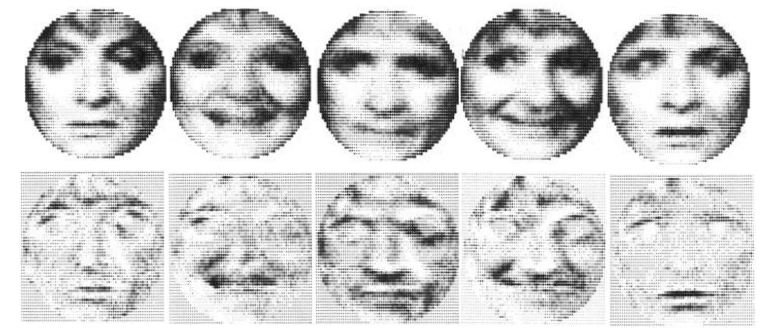
\includegraphics[width=0.8\textwidth]{novelty_faces_cropped.png}
		\caption*{\hspace{5cm} \textit{(taken from Kohonen 1989)}}
	\end{figure}

	\vspace{-0.5cm}
	\begin{itemize}
		\item training data: ''neutral'' facial expressions (not shown here)
		\begin{itemize}
			\itl $\vec{\Phi}$ projects into space orthogonal to this data
		\end{itemize}
		\item top row: faces $\vec{x}^{(\beta)}$ with different expressions
		\item bottom row: projection $\vec{\Phi} \vec{x}^{(\beta)}$
	\end{itemize}

\paragraph{Novelty Filter: Summary}\mbox{}\\
	\textbf{One neuron:}
	\[ \begin{array}{ll}
	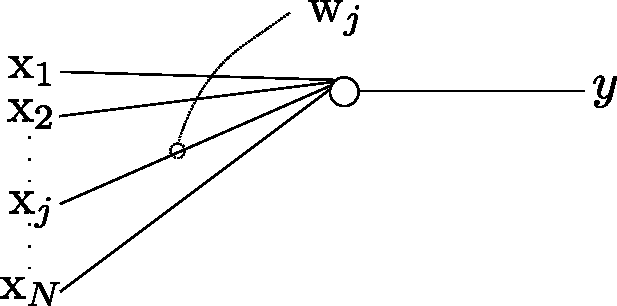
\includegraphics[width=5cm]{section2_fig5}
	& y = \vec{w}^T \vec{x}
	\end{array} \]
	\textbf{Anti-Hebbian learning rule}
		\begin{equation*}
			\Delta \mathrm{w}_j = - \varepsilon y^{(\alpha)} \Bigl\{ \overbrace{\mathrm{x}_j^{(\alpha)}}^{\substack{\text{Anti-Hebbian} \\ \text{learning}}} \underbrace{ - y^{(\alpha)} \mathrm{w}_j \Bigr\} + \varepsilon \Bigl\{ 1- \overbrace{\sum_{k=1}^{N} \mathrm{w}_k^2}^{=\abs{\vec{w}}^2} \Bigr\} \mathrm{w}_j}_{\text{normalization}}
		\end{equation*}
		
\textbf{$N$ neurons:}\\
	\begin{center}
	 \begin{tabular}{ll}
		\includegraphics[width=5.5cm]{section2_fig26}
		& \raisebox{1cm}{$\tilde{\vec{y}}^{(\alpha)} = \vec{\Phi} \vec{x}^{(\alpha)}$}
	\end{tabular} 
	\end{center}
	\textbf{Learning rule:}
		\begin{equation*}
			\Delta \vec{\Phi} = - \varepsilon \vec{\Phi}^2 \vec{x}^{(\alpha)} \left( \vec{x}^{(\alpha)} \right)^T \vec{\Phi}^2
		\end{equation*}
		\vspace{-0.5cm}
		\begin{itemize}
			\itl $\vec{\Phi}$ converges to projection matrix onto subspace orthogonal to training data
		\end{itemize}
		
		
% -----------------------------------------------------------------------------

\newpage 						% for visual reasons
\section{Independent Component Analysis}
% -----------------------------------------------------------------------------
\subsection{Independent Component Analysis}
\label{sec:ICA}
The methods described in this section use a linear generative model to extend decorrelation methods like PCA to find statistically independent sources.\\\\
\textbf{The cocktail party problem:} linear superposition of sources

\begin{figure}[h]
  \centering
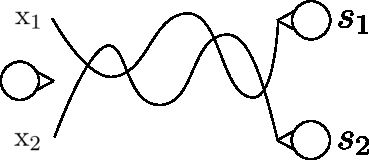
\includegraphics[width=5cm]{section2_fig10}  
\begin{equation}
	\underbrace{ \vec{x} }_{ \text{observations} } 
	= \underbrace{ \vec{A} }_{ \substack{ 	\text{mixing} \\
						\text{matrix}} }
	\underbrace{ \vec{s} }_{ \text{sources} }
\end{equation}

  \caption{The cocktail party problem}
  \label{fig:cocktailParty}
\end{figure}


\paragraph{Question:}
Can we recover the sources from the observations - with no prior knowledge about the mixing process (i.e. the matrix $\vec{A}$)?
\\\\
Yes - but we need to make assumptions about the statistical properties of the sources. 
\begin{itemize}
	\itl source separation methods differ in what prior knowledge they exploit
\end{itemize}

\begin{table}[h]
  \centering
\fbox{
  \begin{tabular}{>{$}c<{$}c c c >{$}c<{$}}
  Approach\; 1 \; \textrm{(direct)}
    && $\vec{x}^{(\alpha)}\; \overset{\mathrm{iid}}{\sim} P_{\vec{x}}(\vec{x})$  
    & &Approach\; 2 \; \textrm{(Infomax)} \\
  & & Data   & &\\ 
  & & $\Downarrow$ & &\\ 
% P_{\vec{s}}(\hat{\vec{s}}),\; \; 
\hat{\vec{s}}:=\vec{W}\, \vec{x}    & & 
  Models & &  \hat{u}_i := \hat f_i( \overbrace{e_i^T\vec{W}\, \vec{x}}^{=: \hat s_i})\\ 
   & & $\Downarrow$ && \\ 
D_\textrm{KL}(P_{\vec{s}}(\hat{\vec{s}}) \; || \; \prod_i P_{s_i}(\hat{s_i}) )   & & Performance measure && H(\hat{\vec{u}})\\ 
   & & $\Downarrow$ && \\ 
\displaystyle \min_{\vec{W}} D_\textrm{KL}   & & Optimization &&  \displaystyle \max_{\vec{W}} H(\hat{\vec{u}})\\ 
  \end{tabular}
}
  \caption{Overview of the 2 approaches: Note that the two approaches are equivalent if the 
  ``transition functions'' $\hat f_i$ match the marginal distribution functions of the 
  true independent sources i.e. $f_i = cdf(s_i)$.}
  \label{tab:approach}
\end{table}

\paragraph{Goal:} recovery of independent sources $\hat{S}$ from observations

\paragraph{Procedure:}
Given observations $\vec{x}$, find $\vec{W}$ with 
\begin{equation}
	\underbrace{ \widehat{\vec{s}} }_{ \substack{ 	\text{''estimated} \\
							\text{sources''}} }
	= \underbrace{ \vec{W} }_{ \substack{	\text{''unmixing} \\
						\text{matrix''}} }
	\underbrace{ \vec{x} }_{ \text{observations} }
\end{equation}
such that the joint distribution of sources factorizes:
\begin{equation}
	P_{\vec{s}} (\widehat{\vec{s}}) 
	= \prod_{i = 1}^N P_{\vec{s}}(\widehat{s_i})
\end{equation}
In the special case of a noise-free mixing process, this means:
\begin{equation}
	\vec{W} = \vec{A}^{-1}
\end{equation}


\paragraph{Why not PCA?} Decorrelation is not independence!

\begin{figure}[h]
  \centering
$P_{\vec{s}}(\vec{s})=P_{s_1}(s_1)\cdot P_{s_2}(s_2)$
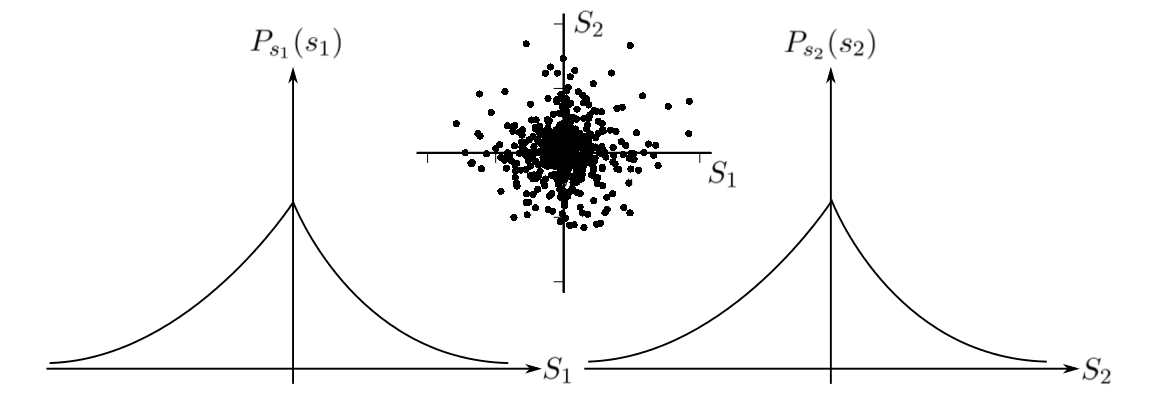
\includegraphics[width=14cm]{section2_fig11mod}  
  \caption{Marginal and joint distribution of independent variables}
  \label{fig:jointMarginal}
\end{figure}


\begin{equation}
	\vec{x} = \vec{A} \vec{s} = \left( \begin{array}{ll}
			a_{11} & a_{12} \\ a_{21} & a_{22}
		\end{array} \right) \cdot \left( \begin{array}{ll}
			s_1 \\ s_2
		\end{array} \right)
	= \left( \begin{array}{l}
		a_{11} s_1 + a_{12} s_2 \\ a_{21} s_1 + a_{22} s_2
	\end{array} \right)
\end{equation}
let $\vec{A} = \big( \vec{a}_1, \vec{a}_2 \big)$:
\begin{equation}
	\begin{array}{ll}
	\vec{s} = \left( \begin{array}{l} 1 \\ 0 \end{array} \right) 
		\leadsto \vec{x} = \left( \begin{array}{l} 
		a_{11} \\ a_{21} \end{array} \right) = \vec{a}_1
		& \text{1st source} 
		\\\\
	\vec{s} = \left( \begin{array}{l} 0 \\ 1 \end{array} \right) 
		\leadsto \vec{x} = \left( \begin{array}{l} 
		a_{12} \\ a_{22} \end{array} \right) = \vec{a}_2
		& \text{2nd source}
	\end{array}
\end{equation}
\begin{figure}[h]
  \centering
  \begin{tabular}{c c}
  \includegraphics[height=4.85cm]{section2_fig12}  &     
  \includegraphics[height=4.8cm]{section2_fig13}
  \end{tabular}
  \caption{Motivation for ICA: In a set of observations, sources are ''interesting'' directions in feature space
    (left). Decorrelation (e.g. through PCA, right), might not find the relevant directions $\Rightarrow$ new  methods needed!}

  \label{fig:icaExample1}
\end{figure}



\paragraph{Limits to recovery}
\begin{enumerate}[(1)]
\item permutations of sources
\begin{equation*}
	\begin{array}{ccc}
	\left( \begin{array}{ll}
		\widehat{s}_1 \\ \widehat{s}_2
	\end{array} \right)
	=
	\left( \begin{array}{ll}
		\mathrm{w}_{11} & \mathrm{w}_{12} \\
		\mathrm{w}_{21} & \mathrm{w}_{22} 
	\end{array} \right)
	\left( \begin{array}{ll}
		\mathrm{x}_1 \\ \mathrm{x}_2
	\end{array} \right)
	& \corresponds &
	\left( \begin{array}{ll}
		\widehat{s}_2 \\ \widehat{s}_1
	\end{array} \right)
	=
	\left( \begin{array}{ll}
		\mathrm{w}_{21} & \mathrm{w}_{22} \\
		\mathrm{w}_{11} & \mathrm{w}_{12} 
	\end{array} \right)
	\left( \begin{array}{ll}
		\mathrm{x}_1 \\ \mathrm{x}_2
	\end{array} \right)
	\\\\
	P_{s_1} (\widehat{s}_1) \cdot P_{s_2} (\widehat{s}_2)
	&& 
	P_{s_2} (\widehat{s}_2) \cdot P_{s_1} (\widehat{s}_1)
	\end{array}
\end{equation*}
\indent both alternatives are solutions to the unmixing problem
\item amplitude of the sources
\begin{equation*}
	\begin{array}{ccc}
	\left( \begin{array}{ll}
		\widehat{s}_1 \\ \widehat{s}_2
	\end{array} \right)
	=
	\left( \begin{array}{ll}
		\mathrm{w}_{11} & \mathrm{w}_{12} \\
		\mathrm{w}_{21} & \mathrm{w}_{22} 
	\end{array} \right)
	\left( \begin{array}{ll}
		\mathrm{x}_1 \\ \mathrm{x}_2
	\end{array} \right)
	& \corresponds &
	\left( \begin{array}{ll}
		a\widehat{s}_1 \\ b\widehat{s}_2
	\end{array} \right)
	=
	\left( \begin{array}{ll}
		a\mathrm{w}_{11} & a\mathrm{w}_{12} \\
		b\mathrm{w}_{21} & b\mathrm{w}_{22} 
	\end{array} \right)
	\left( \begin{array}{ll}
		\mathrm{x}_1 \\ \mathrm{x}_2
	\end{array} \right)
	\\\\
	P_{s_1} (\widehat{s}_1) \cdot P_{s_2} (\widehat{s}_2)
	&& 
	P_{s_1} (a\widehat{s}_1) \cdot P_{s_2} (b\widehat{s}_2)
	\end{array}
\end{equation*}
\indent both alternatives are solutions to the unmixing problem
\\\\
\item Gaussian distributions for sources and observations
\begin{equation*}
	\widehat{\vec{s}} = \vec{W} \vec{x} 
\end{equation*}
Assuming whitened variables, the probability depends only on the length of the vector, i.e.\ distance of the point from the origin. 
\begin{equation}
	\begin{array}{ll}
	P_{\vec{s}}(\widehat{\vec{s}}) 
	& = \frac{1}{2\pi} \exp \bigg\{ -\frac{\widehat{\vec{s}}^2}{2} \bigg\}
	\\\\
	& = \underbrace{ \Bigg[ \frac{1}{\sqrt{2\pi}} \exp \bigg\{ -
		\frac{\widehat{s_1}^2}{2} \bigg\} \Bigg] \Bigg[
			\frac{1}{\sqrt{2\pi}} \exp \bigg\{ -
			\frac{\widehat{s_2}^2}{2} \bigg\}
		\Bigg] }_{\text{solution to the unmixing problem} }
	\end{array}
\end{equation}
\indent let $\vec{B}$ be an orthogonal matrix: $\vec{B}^T \vec{B} = \vec{1}$
\begin{equation}
	\begin{array}{ll}
		\widetilde{\vec{s}} 
		& = \vec{B} \widehat{\vec{s}} \\\\
		& = \vec{B} \vec{W} \vec{x} \\\\
		& = \vec{W'} \vec{x}
	\end{array}
\end{equation}
\begin{equation}
	\begin{array}{ll}
		\widetilde{\vec{s}}^2:=\|\widetilde{\vec{s}}\|_2^2 
		& = \sum\limits_{i = 1}^2 \widetilde{s}_i^2 \\\\
		& = \sum\limits_{i,k,l = 1}^2 B_{ik} \widehat{s}_k B_{il} \widehat{s}_l
			\\\\
		& = \sum\limits_{k,l = 1}^2 \widehat{s}_k
			\bigg( \sum\limits_{i = 1}^2 B_{ki}^T B_{il} \bigg)
			\widehat{s}_l \\\\
		& = \widehat{\vec{s}}^T 
			\underbrace{ \big( \vec{B}^T \vec{B} \big) }_{
				\eqexcl \vec{1} } \widehat{\vec{s}} \\\\
		& = \widehat{\vec{s}}^2
	\end{array}
\end{equation}
\begin{equation}
	\widetilde{\vec{s}} = \vec{W}' \vec{x}
\end{equation}
\begin{equation}
	\begin{array}{ll}
	P_{\vec{s}}(\widetilde{\vec{s}}) 
	& = \frac{1}{2\pi} \exp \bigg\{ -\frac{\widetilde{\vec{s}}^2}{2} \bigg\}
	\\\\
	& = \underbrace{ \Bigg[ \frac{1}{\sqrt{2\pi}} \exp \bigg\{ -
		\frac{\widetilde{s_1}^2}{2} \bigg\} \Bigg] \Bigg[
			\frac{1}{\sqrt{2\pi}} \exp \bigg\{ -
			\frac{\widetilde{s_2}^2}{2} \bigg\}
		\Bigg] }_{\text{also solution to the unmixing problem} }
	\end{array}
\end{equation}
\end{enumerate}
% -----------------------------------------------------------------------------

\subsection[Model-based Source Separation]{Model-based Source Separation Techniques}
\subsubsection{The Infomax Principle}
observations: $\vec{x} \in \mathbb{R}^N, P_{\vec{x}}(\vec{x}) \leftarrow$ true (unknown) density 
\\\\
estimated sources: $\widehat{\vec{s}} = \vec{W} \vec{x}, \widehat{\vec{s}} \in \mathbb{R}^N, \vec{W}$ regular $N \times N$ matrix
\begin{itemize}
	\itl $P_{\vec{s}}(\widehat{\vec{s}})$: family of true (unknown) 
		densities, parametrized by $\vec{W}$
\end{itemize}
\paragraph{Approach 1: direct model selection} (cf. section \ref{sec:ParametricDensityEstimation})
\begin{itemize}
\item[\emph{Idea:}]select the model, which yields a distribution most similar to a factorizing density
\end{itemize}
\begin{equation}
	\widehat{P}_{\vec{s}}(\widehat{\vec{s}}) 
	= \prod_{i = 1}^N \widehat{P}_{s_i}(\widehat{s}_i)
	\leftarrow \text{ ICA assumption}
\end{equation}
This naturally leads to formulation of the following cost function
\begin{equation}
	\dkl = \int d \widehat{\vec{s}} P_{\vec{s}}(\widehat{\vec{s}})
		\ln \frac{P_{\vec{s}}(\widehat{\vec{s}})}{
			\prod_{i = 1}^N \widehat{P}_{s_i}(\widehat{s}_i) }
		\eqexcl \min
\end{equation}
which could be directly optimized. 
But: estimation of $\vec{W} \; \corresponds$ estimation of the probability density $P_{\vec{s}}(\widehat{\vec{s}})$
\begin{itemize}
	\itl parametrized density estimate required (which can be expensive)
\end{itemize}



\paragraph{Approach 2: Information Maximization (Bell \& Sejnowski, 1995)}
\label{sec:ICA-BellSejnowski}
\begin{itemize}
\item[\emph{Idea:}] Under certain conditions, maximizing the
  \emph{mutual information} between inputs (mixed signals) and outputs
  (recovered sources) of a system yields \emph{independent} outputs.\footnote{For a more detailed description of this argument, see \textcite{BellSejnowski1995}.} Note that if sources are independent, then
  transformations of these sources are independent, too.
\item[$\leadsto$] Choosing the transformation in a clever way (such
  that their marginal distributions become uniform, see below)
  simplifies the computations to find independent sources.
\end{itemize}
\emph{Excursion on Density Transformations:} We will see that
computations simplify if we choose a transformation $\widehat{f}_i$
leading to uniformly distributed sources, i.e. $\widehat{u}_i =
\widehat{f}_i(\widehat{s}_i)$, such that
$\widehat{P}_{u_i}(\widehat{u}_i) = \mathrm{const.}$
\\\\
The transformation can be found using \emph{conservation of probability}
\begin{equation}
	\widehat{P}_{u_i}(\widehat{u}_i) d \widehat{u}_i 
	\; =  \; \widehat{P}_{s_i} (\widehat{s}_i) d \widehat{s}_i.
\end{equation}
Using the general rule for density transformations and applying it here yields
\begin{equation}
	\widehat{P}_{u_i}(\widehat{u}_i) \quad
	 =  \quad \bigg| 
		\frac{d \widehat{s}_i}{d \widehat{u}_i} \bigg| 
			 \widehat{P}_{s_i}(\widehat{s}_i) \quad
	 =  \quad \frac{1}{\big| \widehat{f}_i^{'} (\widehat{s}_i) \big|} 
		\widehat{P}_{s_i}(\widehat{s}_i)
\end{equation}
where $\left|\frac{d \widehat{s}_i}{d \widehat{u}_i} \right|$ is
called \emph{functional determinant} of the transformation
$\widehat{f}_i$. For a general transformation, this is illustrated in
figure \ref{fig:densityTransformation}.
\begin{figure}[h]
  \centering
  \includegraphics[width=\linewidth]{section2_fig14}  
  \caption{Illustration of a density transformation}
  \label{fig:densityTransformation}
\end{figure}
Applying the principle of conservation of probability (equal size
areas) to find a transformation resulting in a uniformly distributed
variable with a constant density yields: 
\begin{equation}
  \label{eq:1}
		\widehat{P}_{u_i} (\widehat{u}_i) \; = \;   
		 \frac{1}{\big| \widehat{f}_i^{'} (\widehat{s}_i) \big|} 
		\widehat{P}_{s_i}(\widehat{s}_i) \; \stackrel{!}{=} \; const \qquad \Rightarrow \qquad 
		 \big| \widehat{f}_i^{'} (\widehat{s}_i) \big| =  a \widehat{P}_{s_i}(\widehat{s}_i) 
\end{equation}
and therefore
\begin{equation}
\Rightarrow \widehat{f}_i (\widehat{s}_i)
 = \int\limits_{-\infty}^{\widehat{s}_i} dy\; a 
			\widehat{P}_{s_i}(y)
\end{equation}

\begin{figure}[h]
  \centering
  \includegraphics[width=12cm]{section2_fig15}  
  \caption{density (pdf) and corresponding distribution function (cdf)}
  \label{fig:cdf}
\end{figure}

\paragraph{Application of density transformations to solve the ICA problem:}
\label{sec:appl-dens-transf}
KL-divergence for the transformed densities:
\begin{eqnarray}
  \dkl & = & \int d \vec{s} P_{\widehat{\vec{s}}} \ln \frac{P_{\widehat{\vec{s}}}}{\prod_i P_{\widehat{s_i}}}\\
  & = &  \int d \vec{s} P_{\widehat{\vec{s}}} \ln \frac{P_{\widehat{\vec{s}}} \quad \prod_i \frac{1}{f_i'}}{\prod_i  P_{\widehat{s_i}} \quad \frac{1}{f_i'}}
  \quad = \int d \vec{u} P_{\widehat{\vec{u}}} \ln \frac{P_{\widehat{\vec{u}}}}{\prod_i  P_{\widehat{u_i}}} \\
  & = &  \underbrace{ \int d \widehat{\vec{u}} P_{\vec{u}}
    (\widehat{\vec{u}}) \ln P_{\vec{u}}(\widehat{\vec{u}}) }_{
    \substack{ = -H(u) \\ \text{negative entropy} \\
      \text{of the transformed} \\
      \text{(true) density}} }
  -\int d \widehat{\vec{u}} P_{\vec{u}}
  (\widehat{\vec{u}}) \Bigg(\underbrace{ \ln \prod\limits_{i = 1}^N
    \widehat{P}_{u_i} (\widehat{u}_i)}_{
    \text{const. for 'flat' $u_i$} }\Bigg) 
\end{eqnarray}
This motivates the socalled \emph{Infomax principle} \parencite{BellSejnowski1995}
\begin{equation}\label{eq:infomax}
  H = -\int d \widehat{\vec{u}} P_{\vec{u}} (\widehat{\vec{u}})
  \ln P_{\vec{u}} (\widehat{\vec{u}}) \eqexcl \max 
\end{equation}
using the transformed estimated sources
\begin{equation}
\widehat{u}_i = \widehat{f}_i \big( \underbrace{ \vec{e}_i^T
		\vec{W} \, \vec{x}  }_{= \widehat{s_i} } \big) 
\end{equation}

% -----------------------------------------------------------------------------

\subsubsection{ICA via Neural Networks and Empirical Risk Minimization}
\[ \begin{array}{ll}
	\includegraphics[width=7cm]{section2_fig16}
	& \begin{array}{l}
		\text{perceptron network} \\\\
		u_i = \underbrace{ \widehat{f}_i 
				\Big( \sum\limits_j \mathrm{w}_{ij} 
					\mathrm{x}_j \Big) }_{
					\substack{ \text{often a} \\
						   \text{sigmoid function}} }
				\\\\
		\text{observations: } \vec{x}^{(\alpha)} \in \mathbb{R}^N, 
			\alpha = 1, \ldots, p \\\\
		\rightarrow \substack{	\text{determine the weights} \\
					\text{through inductive learning}}
	\end{array}
\end{array} \]
derivation of the cost function
\begin{equation}
	P_{\vec{u}} (\widehat{\vec{u}}) d \widehat{\vec{u}}
		= P_{\vec{x}}(\vec{x}) d \vec{x}
\end{equation}
\begin{equation}
	\begin{array}{ll}
	P_{\vec{u}} (\widehat{\vec{u}}) 
	& = \left| \frac{d \vec{x}}{d \widehat{\vec{u}}} \right|
		P_{\vec{x}}(\vec{x}) \\\\
	& = \frac{P_{\vec{x}}(\vec{x})}{ \left| 
		\frac{d \widehat{\vec{u}}}{d \vec{x}} \right|}
       = \frac{P_{\vec{x}}(\vec{x})}{|\mathbf{M}|}
	\end{array}
\end{equation}
with elements of the functional determinant $\mathbf{M}$ being given as
\begin{equation}
	\begin{array}{ll}
 \mathbf{M}_{ij}=	\frac{\partial \widehat{u}_i}{\partial \mathrm{x}_j}
	& = \frac{\partial}{\partial \mathrm{x}_j} 
		\widehat{f}_i \bigg( \sum\limits_{k = 1}^N \mathrm{w}_{ik} 
		\mathrm{x}_k \bigg) \\\\
	& = \mathrm{w}_{ij} \widehat{f}_i^{'} \bigg( \sum\limits_{k = 1}^N 
		\mathrm{w}_{ik} \mathrm{x}_k \bigg).
	\end{array}
\end{equation}
We therefore obtain for the value of the functional determinant
\begin{equation} \label{eq:functionalDeterminant}
|\mathbf{M}| = 
	\Big| \frac{\partial \widehat{\vec{u}}}{\partial \vec{x}} \Big|
	= |\vec{w}| \prod\limits_{l = 1}^N  \widehat{f}_l^{'} \Bigg( 
		\sum\limits_{k = 1}^N \mathrm{w}_{lk} \mathrm{x}_k \Bigg).
\end{equation}
Inserting this into the Infomax cost function (\ref{eq:infomax}) gives 
\begin{eqnarray}
H & = & -\int d \widehat{\vec{u}} P_{\vec{u}} (\widehat{\vec{u}})
  \ln P_{\vec{u}} (\widehat{\vec{u}}) \\
& = &  
-\int d \vec{x} P_{\vec{x}} (\vec{x}) \ln \frac{P_{\vec{x}}(\vec{x})}{|\mathbf{M}|} \\
& = & 
\underbrace{-\int d \vec{x} P_{\vec{x}} (\vec{x}) \ln P_{\vec{x}}(\vec{x})}_{ \text{constant w.r.t. } \vec{w} } +
\int d \vec{x} P_{\vec{x}} (\vec{x}) \ln |\mathbf{M}|
\end{eqnarray}
and with~(\ref{eq:functionalDeterminant}) can be written in terms explicitly depending on w:
\begin{equation}
	H = const + \int d \vec{x} P_{\vec{x}} (\vec{x}) \ln |\vec{w}|
		+ \int d \vec{x} P_{\vec{x}} (\vec{x}) \sum\limits_{l = 1}^N
			\ln \widehat{f}_l^{'} \Bigg( \sum\limits_{k = 1}^N 
			\mathrm{w}_{lk} \mathrm{x}_k \Bigg).
\end{equation}
As mentioned above, the entropy can then be used for model selection:
\begin{equation} \tag{generalization cost}
	E^G = \ln |\vec{w}| + \int d \vec{x} P_{\vec{x}} (\vec{x})
		\Bigg\{ \sum\limits_{l = 1}^N \ln
			\widehat{f}_l^{'} \Bigg( \sum\limits_{k = 1}^N 
			\mathrm{w}_{lk} \mathrm{x}_k \Bigg)
		\Bigg\}
\end{equation}
Via the \emph{principle of empirical risk minimization}
\begin{center}
mathematical expectation $E^G \longrightarrow$ empirical average $E^T$
\end{center}
the \emph{training cost}
\begin{equation} \label{eq:trainingCost}
	E^T = \ln |\vec{w}| + \frac{1}{p} \sum\limits_{\alpha = 1}^p
		\sum\limits_{l = 1}^N \ln \widehat{f}_l^{'} \Bigg( 
		\sum\limits_{k = 1}^N \mathrm{w}_{lk} 
		\mathrm{x}_k^{(\alpha)} \Bigg)
\end{equation}
can be used for model selection using empirical data 
\begin{equation}
	\fbox{$ E^T \eqexcl \max $}
\end{equation}

% -----------------------------------------------------------------------------

\subsubsection{Learning by Gradient Ascent}
Model parameters can be optimized by stepwise adustment along the direction of the gradient of the cost function. 

\begin{figure}[h]
  \centering
  \begin{tabular}[c c]{c c}
   \includegraphics[width=7cm]{section2_fig17}
  &\raisebox{2cm}{$\Delta \mathrm{w}_{ij} = \underbrace{ \eta }_{
    \substack{ \text{learning} \\ \text{step}} }
  \frac{\partial E^T}{\partial \mathrm{w}_{ij}}$}
  \end{tabular}  
  \caption{Gradient descent using the training cost}
  \label{fig:gradientDescent}
\end{figure}
\noindent Taking partial derivatives of the training cost (\ref{eq:trainingCost}) wrt. the model parameters $w_{ij}$ yields
\begin{equation}
	\frac{\partial E^T}{\partial \mathrm{w}_{ij}}
	= \underbrace{ \frac{1}{p} \sum\limits_{\alpha = 1}^p 
		\sum\limits_{l = 1}^N \frac{\partial}{\partial \mathrm{w}_{ij}}
		\Bigg\{ \ln \widehat{f}_l^{'} \Bigg( \sum\limits_{k = 1}^N 
		\mathrm{w}_{lk} \mathrm{x}_k^{(\alpha)} \Bigg) \Bigg\} }_{
			\frac{1}{p} \sum\limits_{\alpha = 1}^p 
			\frac{ \widehat{f}_i^{''} \Big( \sum\limits_{k = 1}^N 
				\mathrm{w}_{ik} \mathrm{x}_k^{(\alpha)} \Big)
			}{\widehat{f}_i^{'} \Big( \sum\limits_{k = 1}^N 
			\mathrm{w}_{ik} \mathrm{x}_k^{(\alpha)} \Big)}
			\cdot \mathrm{x}_j^{(\alpha)} }
		+ \underbrace{ \frac{\partial}{\partial \mathrm{w}_{ij}}
			\big( \ln |\vec{w}| \big) }_{
				\big( \vec{w}^{-1} \big)_{ji} }
\end{equation}
with individual costs:
\begin{equation}
	e^{(\alpha)} = \ln |\vec{w}| + \sum\limits_{l = 1}^N \ln
		\widehat{f}_l^{'} \Bigg( \sum\limits_{k = 1}^N 
		\mathrm{w}_{lk} \mathrm{x}_k^{(\alpha)} \Bigg)
\end{equation}
\begin{equation}
	\frac{\partial e^{(\alpha)}}{\partial \mathrm{w}_{ij}}
	= \underbrace{ \big( \vec{w}^{-1} \big)_{ji} }_{
		\substack{ \text{costly} \\ \text{computation}} }
		+ \underbrace{  
			\frac{ \widehat{f}_i^{''} \bigg( \sum\limits_{k = 1}^N 
				\mathrm{w}_{ik} \mathrm{x}_k^{(\alpha)} \bigg)
			}{\widehat{f}_i^{'} \bigg( \sum\limits_{k = 1}^N 
			\mathrm{w}_{ik} \mathrm{x}_k^{(\alpha)} \bigg)}
			 }_{ \coloneqq \varphi_i^{(\alpha)} }
		\cdot \mathrm{x}_j^{(\alpha)}
\end{equation}
this can be used for \emph{batch-learning}:
\begin{equation}
	\Delta \mathrm{w}_{ij}
	= \frac{\eta}{p} \sum\limits_{\alpha = 1}^p 
	\frac{\partial e^{(\alpha)}}{\partial \mathrm{w}_{ij}}
\end{equation}
or using \emph{on-line-learning} (see algorithm~\ref{alg:onlineGD}).\footnote{see also MI I, chapters 1.3.4 and 1.4.1-1.4.3}
\begin{algorithm}
  \DontPrintSemicolon
  $t \leftarrow 1$\;
  random initialization of weights $w_{ij}$\;
  \Begin{
    $\eta_t = \frac{\eta_0}{t}$\;
    select next data point $\vec{x}^{(\alpha)}$\;
    change all  $\mathrm{w}_{ij}$ according to:
    $\Delta \mathrm{w}_{ij}^{(t)} = \eta_t \frac{\partial e_t^{(\alpha)}}{\partial
	\mathrm{w}_{ij}} $\;
    $t \leftarrow t + 1$}
\caption{On-line learning for ICA}
\label{alg:onlineGD}
\end{algorithm}

% -----------------------------------------------------------------------------

\subsubsection{Natural Gradient Learning}
\textcite{Amari1998} describes a particularly efficient gradient descent algorithm to optimize the ICA-cost function. For details regarding the underlying theoretical framework, see \textcite{AmariEtAl2007}.\\\\
linear transformations: $d \vec{w}, \vec{w}$
\begin{figure}[h]
  \centering
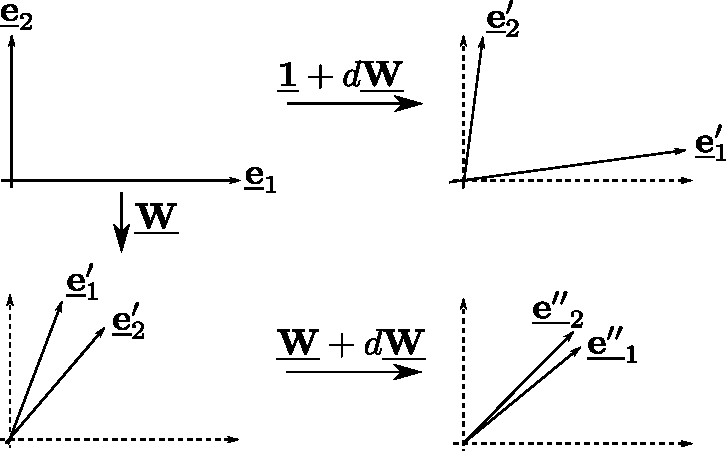
\includegraphics[width=10cm]{section2_fig18}  
  \caption{Illustration of gradient descent in transformed coordinate system}
  \label{fig:NatGrad}
\end{figure}
\begin{equation}
	d \vec{Z} = \underbrace{ d \vec{w} }_{ \text{then do } d \vec{w} }
	\cdot \underbrace{ \vec{w}^{-1} }_{ \substack{
		\text{transfer back to } \vec{1} \\
		\Rightarrow \text{ makes learning} \\
		\text{steps ''comparable''}} }
\end{equation}
This allows to do steepest ascent under normalized step size:
\\\\
Taylor-expansion of $e$ ($e^{(\alpha)}$ but $\alpha$ supressed in the
following):
\begin{eqnarray}
  e_{(\vec{w} + d \vec{w})} & = & e_{(\vec{w})} + \nabla e_{(\vec{w})}^T dw \\
  & = & e_{(\vec{w})} 
  + \underbrace{ \eta }_{ d \vec{w} = \eta \vec{z}_{\mathrm{w}} }
  \big[ \nabla e_{(\vec{w})} \big]^T \cdot \underbrace{ \vec{z}_{
      \mathrm{w}} }_{
     d\vec{w} = \eta \vec{z}_{\mathrm{w}} }
\end{eqnarray}
learning step:
\begin{equation}
	\begin{array}{ll}
		d \vec{Z} 
		& = d \vec{w} \cdot \vec{w}^{-1} \\\\
		& = \eta \vec{z}_{\mathrm{w}} \cdot \vec{w}^{-1}
	\end{array}
\end{equation}
direction of steepest ascent under normalized step-size:
\begin{equation}
	\big[ \nabla e_{(\vec{w})} \big]^T \vec{z}_{\mathrm{w}} 
	\eqexcl \max
\end{equation}
\begin{equation}
	\Big( \vec{z}_{\mathrm{w}} \cdot \vec{w}^{-1} \Big)^2 \eqexcl 1
\end{equation}
The solution for $z_{ij}$ can be found using Lagrange multipliers:
\begin{equation}
	\sum\limits_{i,j = 1}^N \frac{\partial e}{\partial \mathrm{w}_{ij}}
	\big( \vec{z}_{\mathrm{w}} \big)_{ij} - \lambda 
	\sum\limits_{i,j,k,l = 1}^N \big( \vec{z}_{\mathrm{w}} \big)_{ij}
	\big( \vec{w}^{-1} \big)_{jl} \big( \vec{z}_{\mathrm{w}} \big)_{ik}
	\big( \vec{w}^{-1} \big)_{kl} \eqexcl \max
\end{equation}
taking the derivative wrt.\ the $z_{\gamma,s}$ and setting to zero yields
\begin{equation}
	\frac{\partial e}{\partial w_{\gamma s}} - 2 \lambda
	\sum\limits_{k = 1}^N \big( \vec{z}_{\mathrm{w}} \big)_{\gamma k}
	\sum\limits_{l = 1}^N \big( \vec{w}^{-1} \big)_{kl} 
	\big( \vec{w}^{-1} \big)_{ls} \eqexcl 0
\end{equation}
\begin{equation}
	\frac{\partial e}{\partial \vec{w}} = 2 \lambda \vec{z}_{\mathrm{w}}
	\vec{w}^{-1} \big( \vec{w}^{-1} \big)^T
\end{equation}
\begin{equation}
	\vec{z}_{\mathrm{w}} = \frac{1}{2\lambda} \frac{\partial e}{\partial
		\vec{w}} \vec{w}^T \vec{w}
\end{equation}
yielding the direction for ''natural'' gradient ascent
\begin{equation}
	\Delta \vec{w} = \eta \frac{ \overbrace{\partial e}^{
		\substack{	\text{''original''} \\ 
				\text{gradient}} }}{\partial \vec{w}}
		\underbrace{ \vec{w}^T \vec{w} }_{
			\substack{	\text{normalization} \\
					\text{of step size}} }
\end{equation}
\begin{equation} \label{eq:natgrad2}
	\fbox{$ \Delta \mathrm{w}_{ij} = \eta \sum\limits_{l = 1}^N
	\left\{ \delta_{il} 
	+ \frac{ \widehat{f}_i^{''} \Big( \sum\limits_{k = 1}^N 
			\mathrm{w}_{ik} \mathrm{x}_k^{(\alpha)} \Big)
			}{\widehat{f}_i^{'} \Big( \sum\limits_{k = 1}^N 
			\mathrm{w}_{ik} \mathrm{x}_k^{(\alpha)} \Big)}
	\sum\limits_{k = 1}^N \mathrm{w}_{lk} \mathrm{x}_k^{(\alpha)}
	\right\} \mathrm{w}_{lj}
	$}
\end{equation}
\begin{itemize}
\item efficient \& fast learning rule (no matrix inversions
  necessary!)
\item this normalization of stepsize is equivalent to imposing a
  Riemannian metric (with metric tensor $\vec{G} = \vec{w}^{-1} \cdot
  \vec{w}^T$) on space of $\vec{w}$'s
\end{itemize}
% -----------------------------------------------------------------------------

\subsubsection{Some Practical Aspects}
\paragraph{(1) undetermined source amplitudes $\leadsto$ convergence problems}
\mbox{}\\\\
Bell-Sejnowski solution:
\begin{equation}
	\Delta \mathrm{w}_{ii} = 0 \text{ and } \mathrm{w}_{ii} = 1 
	\text{ for all } i
\end{equation}
Amari solution: Learning steps always orthogonal to subspace of
equivalent unmixing matrices.
\begin{equation}
	\Delta \mathrm{w}_{ij} = \eta \frac{ \widehat{f}_i^{''} \bigg( 
		\sum\limits_{k = 1}^N 
		\mathrm{w}_{ik} \mathrm{x}_k^{(\alpha)} \bigg)
		}{\widehat{f}_i^{'} \bigg( \sum\limits_{k = 1}^N 
		\mathrm{w}_{ik} \mathrm{x}_k^{(\alpha)} \bigg)}
		\sum\limits_{l \neq i}^N \Bigg( \sum\limits_{k = 1}^N
		\mathrm{w}_{lk} \mathrm{x}_k^{(\alpha)} \Bigg)
		\mathrm{w}_{lj}
\end{equation}

\paragraph{(2) choice of $\widehat{f}_i$ : true distribution is typically unknown} \mbox{} \\\\
Idea: probability density with one maximum is very likely $\leadsto$ cdf will be roughly sigmoidal
\\\\
typical choice:
\begin{equation} \tag{logistic function}
	\widehat{f}_{(y)} = \frac{1}{1 + \exp(-y)}
\end{equation}
\begin{equation}
	\frac{\widehat{f}_{(y)}^{''}}{\widehat{f}_{(y)}^{'}}
	= 1 - 2 \widehat{f}_{(y)}
\end{equation}
Observation: ICA is fairly robust against false choice of $\widehat{f}$. \\\\
Ansatz: Ignoring scaling of $\hat{s}_i$, i.e.\ using (\ref{eq:natgrad2}):
for stationary state of natural gradient ascent (batch) the following has to hold:
\begin{equation}
	\Delta \vec{w}_{ij} \eqexcl 0
\end{equation}
\begin{equation}
	\delta_{il} \eqexcl -\frac{1}{p} \sum\limits_{\alpha = 1}^p 
	\underbrace{ \frac{ \widehat{f}_i^{''} \bigg( 
		\sum\limits_{k = 1}^N 
		\mathrm{w}_{ik} \mathrm{x}_k^{(\alpha)} \bigg)
		}{\widehat{f}_i^{'} \bigg( \sum\limits_{k = 1}^N 
		\mathrm{w}_{ik} \mathrm{x}_k^{(\alpha)} \bigg)} }_{
			\varphi_i \big( \widehat{s}_i^{(\alpha)} \big) }
	\cdot \underbrace{ \sum\limits_{k = 1}^N \mathrm{w}_{lk} 
		\mathrm{x}_k^{(\alpha)} }_{
			\widehat{s}_l^{(\alpha)} }
\end{equation}
Ansatz: $\widehat{s}_i = \lambda_i s_i$ estimated $\sim$ true source signal\\\\
\indent $i = l$:
\begin{equation}
	-\frac{1}{p} \sum\limits_{\alpha = 1}^p \varphi_i \Big(
		\widehat{s}_i^{(\alpha)} \Big) \lambda_i s_i^{(\alpha)} 
		\eqexcl 1
\end{equation}
As $\lambda$ is a free parameter, this condition can always be fulfilled through proper choice of $\lambda_i$. \\\\
For $i \neq l$ and in the limit of large number of observations:
\begin{equation}
\delta_{il}	\frac{1}{p} \sum\limits_{\alpha = 1}^p \varphi_i \Big(
		\widehat{s}_i^{(\alpha)} \Big) \lambda_l s_l^{(\alpha)}
	\rightarrow \bigg< \varphi_i \Big(
		\widehat{s}_i^{(\alpha)} \Big) \lambda_l s_l^{(\alpha)}
		\bigg>_{P_{\vec{s}}}
\end{equation}
\begin{equation}
	\Big< \varphi_i \big( \lambda_i s_i \big) \lambda_l s_l \Big>
	\underbrace{ = }_{ \substack{ 	\text{statistical} \\
					\text{independence}} }
	\Big< \varphi_i \big( \lambda_i s_i \big) \Big>
	\Big< \lambda_l s_l \Big>
	\eqexcl 0
\end{equation}
Can always be fulfilled if data is ''centered'': $< s_l > = 0$
\\\\
Therefore true (independent) source signals are always a fixed point of the 
natural gradient ascent $\rightarrow$ independent of choice
of $\widehat{f}_i$

\begin{itemize}
	\itR however: if $\widehat{f}_i$ deviates too strongly from its true
		shape, the fixed point may become unstable
	\itR if in doubt (and enough data available)
	\begin{itemize}
		\itl make a parametrized ansatz for $\widehat{f}_i$
		\itl estimate parameters in addition to $\vec{w}$
	\end{itemize}
\end{itemize}

% -----------------------------------------------------------------------------
\newpage
\subsection{Second Order Blind Source Separation}

% -----------------------------------------------------------------------------

% \subsubsection{}
Compared to the estimation of correlations (second order moments), the
estimation of higher order moments from (small) samples of noisy
observations is often unreliable. In such cases, using
additional knowledge about the source signals can be exploited to
extend decorrelation methods and separate sources more robustly.

The following two methods (FFDIAG, QDIAG) exploit the assumption of
finite length \emph{autocorrelations} to implement noise robust
unmixing. Typical examples of such non-iid data displaying temporal
correlation structure include or time series such as videos, EEG, fMRI, MEG data.



\paragraph{2nd order ''separation'' idea:} find an unmixing matrix $\vec{w}$,
such that all cross-correlation functions vanish\footnote{All the
  presented approaches assume a \emph{linear} mixing model, i.e.\
  $\vec{x} \approx \vec{A} \vec{s}$. In many scenarios, this might not
  be a good model. However, for small amplitudes of variation around
  an operating point $\vec{s}_0$ this can still be used as a reasonable
  approximation for the more general relation $\vec{x} = f(\vec{s})$ as $\vec{x} =
  f(\vec{s}_1) = f(\vec{s_0 + \Delta s}) \approx f(\vec{s_0}) + \nabla f(\vec{s_0})  \Delta s$.}
\begin{center}
	statistical independence $\substack{ \text{?} 
		\\ \leftarrow
		\\ \Rightarrow }$ all cross-correlations vanish
\end{center}
\begin{figure}[h]
  \centering
  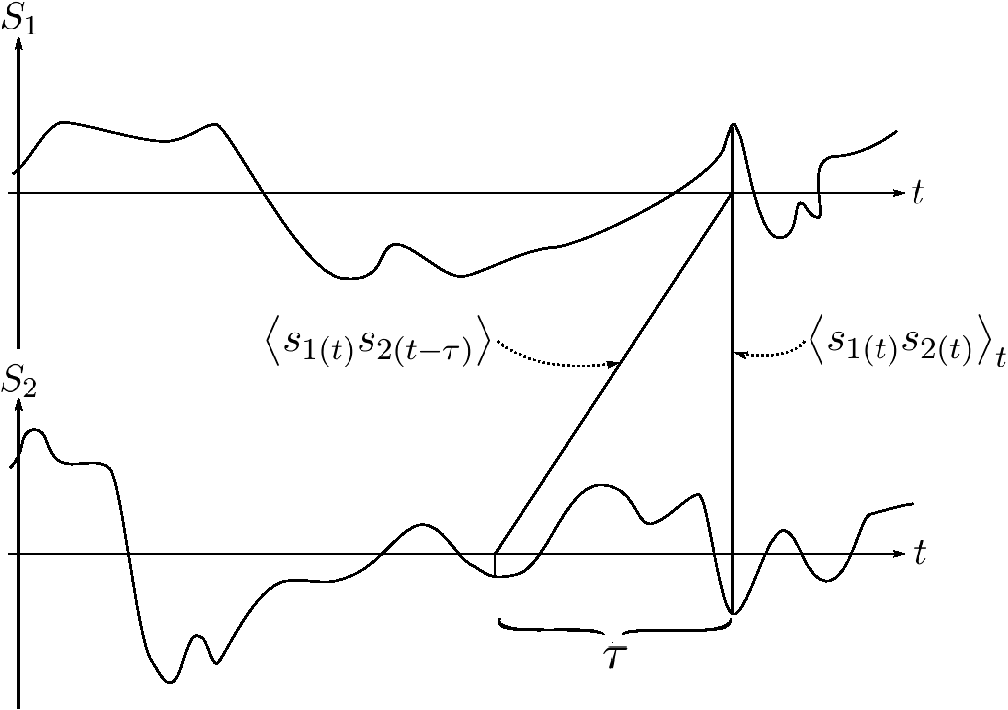
\includegraphics[width=10cm]{section2_fig19}  
  \caption{Source separation for time series data from two sources}
  \label{fig:timeSeriesICA}
\end{figure}


\paragraph{Example: Source separation using two shifts}\mbox{}\\
observations: $\vec{x}_{(t)}$, recorded at different times (from $\vec{x} = \vec{A} \vec{s}$)
\begin{enumerate}[(1)]
\item PCA and sphering
\begin{itemize}
	\itl ''centering'' of the data: $<\vec{x}> = \vec{0}$ \\
		usefull preprocessing for all ICA methods (often including
		dimension reduction)
	\itl solve the eigenvalue problem
	\begin{equation}
		\vec{C}_{\mathrm{x}}^{(0)} \vec{e}_k = \lambda_k \vec{e}_k
		\text{ with } \big[ \vec{C}_{\mathrm{x}}^{
			\overbrace{ (0) }^{ \tau = 0 } 
			} \big]_{ij}
		= \Big< \mathrm{x}_{i (t)} \mathrm{x}_{j (t)} \Big>_t
	\end{equation}
	\itl transformation into the eigenbasis and sphering
	\begin{equation}\label{sec:sphering}
		\vec{M}_0 = \underbrace{ \vec{\Lambda}_0^{-1} }_{
			\substack{	\text{diagonal matrix of} \\
					\text{inverse eigenvalues}} } \cdot
			\underbrace{ \vec{E}_0 }_{
				\substack{	\text{matrix of} \\
						\text{eigenvectors}} }
	\end{equation}
	\begin{equation}
		\vec{u} = \vec{M}_0 \vec{x}
	\end{equation}	
\end{itemize}
\item source separation requires one additional orthogonal transformation
\begin{itemize}
	\itl Ansatz: $\underbrace{ \vec{s} }_{ 
		\substack{ \text{true sources} \\ \text{(independent)}} }
		= \vec{B} \vec{u}$
	\itl for statistically independent sources we obtain
	\begin{equation}
		\begin{array}{lcl}
		\big< s_{i (t)} s_{j (t)} \big>_t 
		& \underbrace{ = }_{ \substack{	\text{statistical} \\
						\text{independence}} } 
				& \delta_{ij} \\\\
		& = & \sum\limits_{k,l = 1}^N B_{ik} \underbrace{
			\big< u_{k (t)} u_{l (t)} \big>_t }_{
				\substack{ \eqexcl \delta_{kl} \\
					\text{({\it cf. sphering})}} } 
			B_{lj}^T \\\\
		& = & \sum\limits_{k = 1}^N B_{ik} B_{kj}^T
		\end{array}
	\end{equation}
	\begin{equation}
		\vec{B} \cdot \vec{B}^T = \vec{1} \leadsto
		\text{orthogonal transformation}
	\end{equation}
\end{itemize}
\item determination of $\vec{B}$ through diagonalization of a time-shifted cross-correlation matrix
\begin{itemize}
	\itl solve the eigenvalue problem
	\begin{equation}
		\vec{C}_u^{(\tau)} \vec{e}_k = \lambda_k \vec{e}_k 
		\text{ with } \Big[ \vec{C}_u^{(\tau)} \Big]_{ij}
		= \Big< u_{i(t)} u_{j(t-\tau)} \Big>_t
	\end{equation}
	\itl transformation into the eigenbasis
	\begin{equation}\label{eq:EVshift}
		\widehat{\vec{s}} = \underbrace{\vec{E}_{  \tau }}_{
			\substack{ \text{matrix of} \\ \text{eigenvectors}} }
			\vec{u}
	\end{equation}
\end{itemize}
\end{enumerate}
\emph{Note:} The matrix of Eigenvectors is orthonormal
($\vec{E}^T_\tau\vec{E}_\tau=\vec{I}$) and therefore a candidate for $\vec{B}$. Combining equations (\ref{sec:sphering}) and (\ref{eq:EVshift}), this gives the transformation 
\begin{equation}
  \label{eq:2ndOrder}
\widehat{\vec{s}} = \vec{E}_\tau \vec{\Lambda}^{-1/2}_0 \vec{E}_0^T \vec{x}
\end{equation}

\paragraph{Noise robust algorithms in the general case:}
Given a set of $T$ zero-mean observations: $\vec{x}_{(t)}$ and corresponding 
number of $N$x$N$ covariance matrices indexed by $\tau$ 
\begin{equation}
	\Big[\vec{C}_{\mathrm{x}}^{(\tau)}\Big]_{ij} = 
	\frac{1}{T} \sum\limits_{t = 0}^{T-1} \mathrm{x}_{i(t)}
	\mathrm{x}_{j(t-\tau)}
\end{equation}
\begin{itemize}
	\item joint diagonalization of multiple cross-correlation matrices
	\item real world data: noise, approximate independence only
	$\leadsto$ only approximate diagonalization possible
	\item disturbances due to sensor noise can be minimized by ommitting $\tau = 0$
\end{itemize}
The following two algorithms implement these ideas using slightly different cost-functions. Both of them are implemented in the \texttt{jointDiag} package, available from CRAN.\footnote{\url{www.cran.r-project.org/web/packages/jointDiag/index.html}}

In order to find an $N \times N$ matrix $\vec{W}$ that diagonalizes the set of the matrices $\vec{C}^{(\tau)}, \tau = 0, 1, ...$ in a
least squares sense, we consider a cost function given by the squared sum of all off-diagonal elements
of $\vec{W} \vec{C}^{(\tau)} \vec{W}^T$. 


\begin{enumerate}[(1)]
\item QDIAG-algorithm
\\\\
\emph{cost function:} squared sum of non-diagonal elements:
\begin{equation}
	E_{[\vec{W}]}^T = \sum\limits_{\tau} \underbrace{ \alpha_\tau }_{
		\substack{ 	\text{weighting} \\ 
				\text{factors} \\
				\text{(optional)}} }
		\sum\limits_{i \neq j} \Big( \vec{W} \vec{C}_{\mathrm{x}}^{(\tau)} \vec{W}^T \Big)_{ij}^2
\end{equation}
\emph{optimization problem:}
\begin{equation}
	\begin{array}{rll}
		E_{[\vec{W}]}^T & \eqexcl \min 
		& \text{minimize cross-correlations} \\\\
		\Big( \vec{W} \vec{C}_{\mathrm{x}}^{(0)} \vec{W}^T \Big)_{ii}
			& = 1 \text{ for all } i
		& \text{avoid trivial solutions}
	\end{array}
\end{equation}
\emph{Comments:}
\begin{itemize}
\item \emph{documentation:} \textcite{VollgrafObermayer2006}, Matlab-code implementing the algorithm can be found on the NI-website\footnote{\url{www.ni.tu-berlin.de/menue/software/approximate_simultaneous_matrix_diagonalization_qdiag/}}
\item \emph{computational complexity:} two versions with complexity
	$O (k \cdot N^3)$ or $O (N^5)$
\item allows for arbitrary (rectangular) matrices $\vec{W}$
\end{itemize}

\item  FFDIAG-algorithm
\\\\
\emph{cost function:} equally weighted
\begin{equation}
	E_{[\vec{W}]}^T = \sum\limits_\tau \sum\limits_{i \neq j}
	\big( \vec{W} \vec{C}_{\mathrm{x}}^{(\tau)} \vec{W}^T \big)_{ij}^2
\end{equation}
\emph{optimization problem:}
\begin{equation}
	\begin{array}{ll}
		E_{[\vec{W}]}^T \eqexcl \min 
		& \text{minimize cross-correlation} \\\\
		\text{invertability of } \vec{W}
		& \text{to avoid trivial solutions}
	\end{array}
\end{equation}
\emph{Comments:}
\begin{itemize}
\item \emph{Documentation:} \textcite{ZieheEtAl2004} 
  \item computational complexity: $O (K \cdot N^2)$ (approaching $O (N^3)$ for large $N$) 
 requires square matrices $\vec{W}$, no weighting
\end{itemize}
\end{enumerate}
Preference for one or the other algorithm depends on problem size and kind of data (cf. \cite{StetterEtAl2000}), \slideref{Ex: optical imaging}

% -----------------------------------------------------------------------------

\subsection{Fast ICA}

\paragraph{ICA and Projection Pursuit}
''interesting'' complex features
\begin{itemize}
	\itl variance criterion $\Rightarrow$ PCA \\
		important preprocessing method, but: scale sensitive solutions
	\itl higher moments: ok, but: Why not maximize non-Gaussianity?
\end{itemize}
ICA and non-Gaussianity
\[ \begin{array}{lc}
	\vec{x} = \vec{A} \vec{s} 
	& \substack{ 	\text{mixing matrix } \vec{A} \text{, statistically} \\
		\text{independent sources}} \\\\
	\widehat{s}_i = \vec{w}_i^T \vec{x}
	& \substack{ 	\text{extraction of one source through one} \\
			\text{row vector of an unmixing matrix}} \\\\
	\widehat{s}_i = \underbrace{ \vec{w}_i^T \vec{A} }_{ \vec{z}_i^T }
		\vec{s} = \vec{z}_i^T \vec{s}
	& \substack{ 	\text{linear combination of statistically} \\
			\text{independent variables}}
\end{array} \]
''The sum of independent random variables is 'more Gaussian' then the original variables''
\begin{itemize}
	\itR interesting directions (projection pursuit) and individual 
		components (ICA) can be extracted by maximizing non-Gaussianity
		w.r.t $\vec{w}$
\end{itemize}

\paragraph{Measures for non-Gaussianity:} The Gaussian is fully characterized by its first and second moments. Deviations from Gaussianity can therefore be quantified via the following measures:
\begin{enumerate}[(1)]
\item Kurtosis
\begin{equation}
	\kurt(u) = \big< u^4 \big>_{P_u (u)} - 3 \underbrace{
		\Big( \big< u^2 \big>_{P_u (u)} \Big)^2 }_{
			\substack{	\text{would be } 1 \text{ for} \\
					\text{sphered data}}}
\end{equation}
\[ \begin{array}{lll}
	\kurt(u) = 0 & \text{Gaussian PDF} 
		& 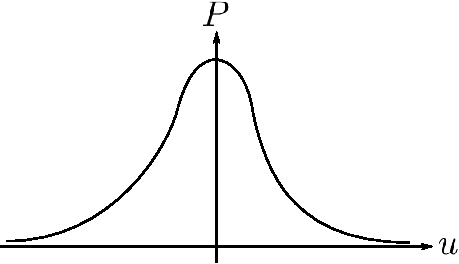
\includegraphics[width=4cm]{section2_fig20}
		\\\\
	\kurt(u) > 0 & \text{''super''-Gaussian PDF}		
		& \includegraphics[width=4cm]{section2_fig21} \\
		& \rightarrow \text{ peaky, long tails (i.e. ''outliers'')} \\
		& \rightarrow \text{ e.g.: Laplace distribution} \\\\
	\kurt(u) < 0 & \text{''sub''-Gaussian PDF}
		& 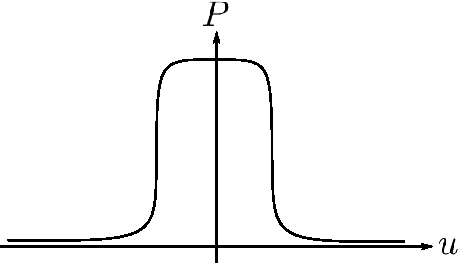
\includegraphics[width=4cm]{section2_fig22} \\
		& \rightarrow \text{ bulky, no ''outliers''} \\
		& \rightarrow \text{ e.g. constant distribution}
\end{array} \]
for independent random variables $u_1$ and $u_2$ we get:
\begin{equation}
	\begin{array}{rl}
		\kurt(u_1 + u_2) 
			& = \kurt(u_1) + \kurt(u_2) \\\\
		\kurt(z_1 u_1)
			& = z_1^4 \kurt(u_1)
	\end{array}
\end{equation}
\emph{Example:} two statistically independent sources with $\big< s_i s_j \big> = \delta_{ij}$
\begin{equation}
	\begin{array}{ll}
		\widehat{s} & = \vec{z}^T \vec{s} \\\\
			    & = z_1 s_1 + z_2 s_2
	\end{array}
\end{equation}
\begin{equation}
	\begin{array}{ll}
		\var(\widehat{s}) 
		& = \Big< \big( z_1 s_1 + z_2 s_2 \big)^2 \Big>_{P_s (s)} \\\\
		& = z_1^2 \big< s_1^2 \big> + z_2^2 \big< s_2^2 \big> \\\\
		& = z_1^2 + z_2^2
	\end{array}
\end{equation}
\begin{equation}
	\kurt(\widehat{s}) = z_1^4 \kurt(s_1) + z_2^4 \kurt(s_2)
\end{equation}
search for ''interesting'' directions
\begin{equation}
	\begin{array}{rllc}
	\kurt(\widehat{s}) & \eqexcl \max_{\vec{z}} 
	& \leftarrow & \substack{ 	\text{search for the direction} \\
					\text{of optimal kurtosis}} \\\\
	z_1^2 + z_2^2 & \eqexcl 1
	& \leftarrow & \substack{	\text{such that data} \\
					\text{remained sphered}}
	\end{array} 
\end{equation}
\emph{Result:} ({\it see supplementary material})
\begin{equation}
	\vec{z} = \left( \begin{array}{c}
			0 \\ \pm 1 
		\end{array} \right)
	\text{ or } 
	\vec{z} = \left( \begin{array}{c}
			\pm 1 \\ 0 
		\end{array} \right)
\end{equation}
independent sources correspond to extrema of the kurtosis
\item Negentropy
\begin{equation}
	J_{(u)} \coloneqq \underbrace{ H_{(u)}^{\mathrm{Gauss}} }_{
			\substack{ 	\text{entropy of Gaussian} \\
					\text{with variance } \sigma^2} }
		- \underbrace{ H_{(u)} }_{
			\substack{	\text{entropy of true} \\
					\text{distribution} \\
					\text{(variance } \sigma^2 \text{)} }}
\end{equation}
\begin{itemize}
	\item interesting, theoretically well founded measure
	\item but: hard to evaluate, optimization is computationally expensive (depends on full distribution)
\end{itemize}
\item Approximations to the negentropy
\begin{equation}
	J_{(u)} \approx \sum\limits_{i = 1}^l \underbrace{ k_i }_{
		\substack{	\text{some} \\ \text{constant}} }
		\bigg\{ \Big< G_{(u)} \Big>_{ \underbrace{ P_u (u) }_{
			\substack{ \text{true} \\ \text{density} } } }
		- \Big< G_{(u)} \Big>_{ \underbrace{ \mathrm{Gauss} }_{
			\substack{ 	\text{reference:} \\
					\text{Gaussian} \\
					\text{density with} \\
					\text{some variance}} } } \bigg\}
\end{equation}
common contrast functions:
\[ \begin{array}{lc}
	G_{1(u)} = \frac{1}{a} \log \cosh a u 
	& \substack{ 	\text{good general purpose function} } \\\\
	G_{2(u)} = -\exp \Big( -\frac{u^2}{2} \Big) 
	& \substack{	\text{good only if sources are} \\
			\text{highly ''super''-Gaussian} \\
			\text{i.e. many outliers} } \\\\
	G_{3(u)} = \frac{1}{4} u^4
	& \substack{	\text{kurtosis (see \textcircled{1}),} \\
			\text{useful if components} \\
			\text{are ''sub''-Gaussian} \\
			\text{i.e. few outliers}}
\end{array} \]
$\leadsto$ Clever choice of $G$ allows to obtain robust approximations to negentropy \textcite{Hyvaerinen1997}, \textcite{HyvaerinenOja2000}. 
\end{enumerate}

\paragraph{Fixed point algorithm for one linear neuron:}
The following algorithm (alg. \ref{alg:fastICA1}) implements \texttt{fastICA} for standardized data (mean=0, sd=1) to learn a single weight vector $\vec{w}$:
\[ \begin{array}{ll}
	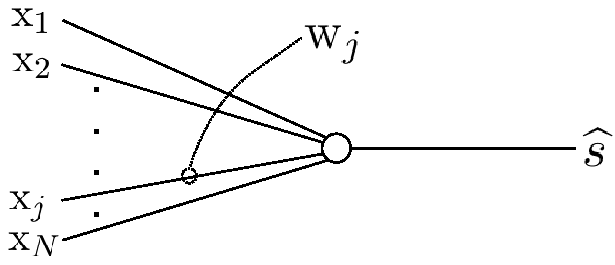
\includegraphics[width=6cm]{section2_fig23}
	& \widehat{s} = \underbrace{ \vec{w}^T }_{ 
		\substack{	\text{''interesting''} \\
				\text{complex} \\
				\text{features}} }
		\vec{x}
\end{array} \]
\begin{algorithm}
  \label{alg:fastICA1}
  \DontPrintSemicolon
  randomly initialize weight vector $\vec{w}$ of unit length\; 
  \Repeat{convergence}{
    \[ \begin{array}{ll}
	\vec{w}^+
	& = \frac{1}{p} \Bigg\{ \sum\limits_{\alpha = 1}^p \vec{x}^{(\alpha)}
		G_{\big( \vec{w}^T \vec{x}^{(\alpha)} \big)}^{'}
		-\vec{w} \sum\limits_{\alpha = 1}^p 
		G_{\big( \vec{w}^T \vec{x}^{(\alpha)} \big)}^{''}
		\Bigg\} \\\\
	\vec{w} 
	& = \frac{\vec{w}^+}{\|\vec{w}^+\|}
\end{array} \]
}
  \caption{fixed-point algorithm for fastICA: single component}
\end{algorithm}
\begin{itemize}
\item for details, see \textcite{Hyvaerinen1999} and \textcite[ch. 8.3.5]{HyvaerinenEtAl2001}.
	\item convergence to direction of extremal ''non-Gaussianity''
	\itR example of a so-called projection pursuit method
\end{itemize}

\paragraph{Fixed-point algorithm for a perceptron}
\[ \begin{array}{ll}
	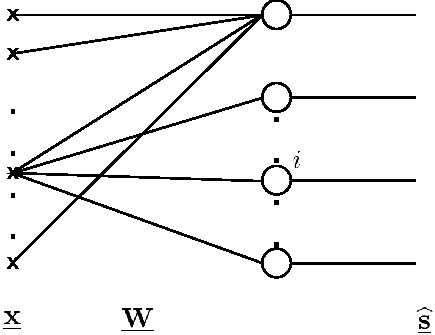
\includegraphics[width=6cm]{section2_fig24}
	& \widehat{\vec{s}} = \vec{W} \vec{x}
\end{array} \]
Algorithm \ref{alg:fastICAN} implements fastICA for standardized data (mean=0, sd=1) to learn the $N \times N$ weight matrix $\vec{W}$.
\begin{algorithm}
  \DontPrintSemicolon
  $t \leftarrow 0$\;
  randomly initialize weight vectors $\vec{w}_i^{(t)}\; \text{for } i \in 1 \dots N$\; 
\Repeat{convergence}{
   symmetric orthogonalization: 
%    $$
%    \vec{W}  \leftarrow \vec{W}/\lVert \vec{W} \rVert \qquad \text{(do not use frobenius norm)}
%    $$
    $$
    \vec{W}^{(t)}  \leftarrow  \frac{3}{2} \vec{W}^{(t)} 
    -  \frac{1}{2} \vec{W}^{(t)} \Big( \vec{W}^{(t)}
    \Big)^T \vec{W}^{(t)}
    $$
     \For{$i \in 1 \dots N$}{
    \begin{eqnarray*}
      \vec{w}_i^{(t)}
      & \leftarrow & \frac{1}{p} \left\{ \sum\limits_{\alpha = 1}^p \vec{x}^{(\alpha)}
        G^{'}\bigg( \big(\vec{w}_i^{(t)}\big)^T \vec{x}^{(\alpha)} \bigg)
        -\vec{w}_i^{(t)} \sum\limits_{\alpha = 1}^p 
        G^{''}\bigg( \big(\vec{w}_i^{(t)}\big)^T \vec{x}^{(\alpha)} \bigg)\right\}\\
      \vec{w}_i^{(t+1)} 	& \leftarrow & \frac{\vec{w}_i^{(t)}}{\| \vec{w}_i^{(t)} \|}
    \end{eqnarray*}
  }
    $t \leftarrow t+1$
  }
  \caption{fixed-point algorithm for fastICA: multiple components}
  \label{alg:fastICAN}
\end{algorithm}
\\\\
\emph{Remark:} The fastICA algorithm can be understood as a fixed point algorithm for maximum likelihood estimation of the ICA-model in which the learning rate for the different directions is adaptively adjusted (see \cite[p. 424]{HyvaerinenOja2000}). For further details, see \textcite[ch. 8.4]{HyvaerinenEtAl2001}. 
\\\\
\emph{code:} \url{http://research.ics.aalto.fi/ica}\\
\slideref{sound demo: blind source separation}
\slideref{natural images: van Hateren and van der Schaaf}

% -----------------------------------------------------------------------------
